\documentclass[a4paper]{article}

%%%%%%%% CREATE DOCUMENT STRUCTURE %%%%%%%%
%% Language and font encodings
\usepackage[english]{babel}
\usepackage[utf8x]{inputenc}
\usepackage[T1]{fontenc}
%\usepackage{subfig}

%% Sets page size and margins
\usepackage[a4paper,top=3cm,bottom=2cm,left=2cm,right=2cm,marginparwidth=1.75cm]{geometry}

%% Useful packages
\usepackage[justification=centering]{caption}
\usepackage{amsmath}
\usepackage{graphicx}
\usepackage[colorlinks=true, allcolors=blue]{hyperref}
\usepackage{sectsty}
\usepackage{cite}
\usepackage{float}
\usepackage{titling} 
\usepackage{blindtext}
\usepackage[colorinlistoftodos]{todonotes}
\usepackage{xcolor}
\usepackage{multirow}
\usepackage{booktabs}
\usepackage{bigstrut}
\usepackage{colortbl}
\usepackage{subfigure} 
\usepackage[section]{placeins}
\definecolor{darkgreen}{rgb}{0.0, 0.4, 0.0}
\setlength{\parskip}{2em}

%%%%%%%% DOCUMENT %%%%%%%%
\begin{document}
%%%% Title Page
\begin{titlepage}

\newcommand{\HRule}{\rule{\linewidth}{0.5mm}} 							% horizontal line and its thickness
\center 
 
% University
\textsc{\LARGE Delft University of Technology}\\[1cm]

% Document info
\textsc{\Large Sensing Technologies and Mathematics for Geomatics}\\[0.2cm]
\textsc{\large GEO1001}\\[1cm] 										% Course Code
\HRule \\[0.8cm]
{ \huge \bfseries Assignment 01: Statistical analysis of a heat stress measurement dataset}\\[0.7cm]								% Assignment
\HRule \\[2cm]
\large
\emph{Authors:}\\
Zhenyu Liu(5386586)\\[1.5cm]													% Author info
{\large \today}\\[5cm]

\includegraphics[width=0.6\textwidth]{images/TU_delft_logo.jpg}\\[1cm] 	% University logo
\vfill 
\end{titlepage}

%%\begin{abstract}
%%Your abstract.
%%\end{abstract}

%%%% SECTIONS
%% Section 1
\section{Runtime environment and source data}
\subsection{Runtime environment}
\noindent All code for this assignment is run using Pycharm on a windows10 64-bit system.The Python version is 3.8.

\subsection{Source data}
\noindent The source data contains 5 different heat stress sensors located in Netherlands. The data is collected from 10-06-2020 to 14-07-2020, contains 20 kinds of data such as \textbf{Wind direction}, \textbf{Wind speed}, \textbf{Crosswind Speed} and \textbf{Headwind Speed}.\cite{Maiullari2020}


\section{Exercises after Lecture A1}
\subsection{Question A1.1}

Computing the mean statistics values(mean, variance and standard deviation for each of the sensors variables), the results are summarized in the following three tables:

% Table generated by Excel2LaTeX from sheet 'mean'
\begin{table}[htbp]
\footnotesize
  \centering
  \caption{The mean value of each variable of the 5 heat stress sensors}
    \begin{tabular}{lrrrrr}
    \toprule
          & \multicolumn{1}{c}{\textbf{A}} & \multicolumn{1}{c}{\textbf{B}} & \multicolumn{1}{c}{\textbf{C}} & \multicolumn{1}{c}{\textbf{D}} & \multicolumn{1}{c}{\textbf{E}} \\
    \midrule
    \textbf{Direction True(°)} & 209.4063 & \cellcolor[rgb]{ .608,  .804,  .608}183.4124 & 183.5889 & 198.3266 & \cellcolor[rgb]{ .98,  .502,  .447}223.9564 \\
    \textbf{Wind Speed(m/s)} & 1.290307 & 1.242124 & 1.371463 & \cellcolor[rgb]{ .98,  .502,  .447}1.581649 & \cellcolor[rgb]{ .608,  .804,  .608}0.596242 \\
    \textbf{Crosswind Speed(m/s)} & 0.964943 & 0.835622 & 0.963298 & \cellcolor[rgb]{ .98,  .502,  .447}1.210509 & \cellcolor[rgb]{ .608,  .804,  .608}0.438505 \\
    \textbf{Headwind Speed(m/s)} & \cellcolor[rgb]{ .98,  .502,  .447}0.16353 & -0.12981 & -0.26289 & \cellcolor[rgb]{ .608,  .804,  .608}-0.30057 & \cellcolor[rgb]{ .98,  .502,  .447}0.194949 \\
    \textbf{Temperature(°C)} & 17.9691 & 18.06543 & \cellcolor[rgb]{ .608,  .804,  .608}17.91314 & 17.99636 & \cellcolor[rgb]{ .98,  .502,  .447}18.35394 \\
    \textbf{Globe Temperature(°C)} & 21.54459 & 21.79943 & 21.58739 & 21.3593 & \cellcolor[rgb]{ .608,  .804,  .608}21.17616 \\
    \textbf{Wind Chill(°C)} & 17.83821 & 17.94592 & \cellcolor[rgb]{ .608,  .804,  .608}17.773 & 17.83537 & \cellcolor[rgb]{ .98,  .502,  .447}18.29402 \\
    \textbf{Relative Humidity(\%)} & 78.18477 & 77.87831 & 77.96285 & 77.94204 & \cellcolor[rgb]{ .608,  .804,  .608}76.79305 \\
    \textbf{Heat Stress Index(°C)} & \cellcolor[rgb]{ .608,  .804,  .608}17.8996 & 18.00428 & 17.82825 & 17.92162 & \cellcolor[rgb]{ .98,  .502,  .447}18.28642 \\
    \textbf{Dew Point(°C)} & 13.55388 & 13.53086 & \cellcolor[rgb]{ .608,  .804,  .608}13.45812 & 13.50861 & \cellcolor[rgb]{ .98,  .502,  .447}13.55879 \\
    \textbf{Psychro Wet Bulb Temperature(°C)} & 15.27072 & 15.29552 & \cellcolor[rgb]{ .608,  .804,  .608}15.19665 & 15.26019 & \cellcolor[rgb]{ .98,  .502,  .447}15.40667 \\
    \textbf{Station Pressure(mb)} & 1016.168 & 1016.657 & 1016.689 & 1016.728 & \cellcolor[rgb]{ .608,  .804,  .608}1016.166 \\
    \textbf{Barometric Pressure(mb)} & \cellcolor[rgb]{ .608,  .804,  .608}1016.128 & 1016.616 & 1016.652 & \cellcolor[rgb]{ .98,  .502,  .447}1016.689 & \cellcolor[rgb]{ .608,  .804,  .608}1016.128 \\
    \textbf{Altitude(m)} & -25.9871 & -30.0582 & -30.3387 & \cellcolor[rgb]{ .608,  .804,  .608}-30.6532 & \cellcolor[rgb]{ .98,  .502,  .447}-25.9612 \\
    \textbf{Density Altitude(m)} & 137.3166 & 135.5808 & \cellcolor[rgb]{ .608,  .804,  .608}129.6229 & 132.4111 & \cellcolor[rgb]{ .98,  .502,  .447}150.84 \\
    \textbf{NA Wet Bulb Temperature(°C)} & 15.98154 & \cellcolor[rgb]{ .98,  .502,  .447}15.99681 & 15.93424 & \cellcolor[rgb]{ .608,  .804,  .608}15.91564 & 15.93689 \\
    \textbf{WBGT(°C)} & 17.25432 & \cellcolor[rgb]{ .98,  .502,  .447}17.32197 & 17.22502 & \cellcolor[rgb]{ .608,  .804,  .608}17.1768 & 17.18554 \\
    \textbf{TWL(w/m\^2)} & 301.3929 & 299.4517 & 301.8998 & \cellcolor[rgb]{ .98,  .502,  .447}305.2546 & \cellcolor[rgb]{ .608,  .804,  .608}284.1153 \\
    \textbf{Direction Mag(°)} & 208.9051 & 183.2173 & \cellcolor[rgb]{ .608,  .804,  .608}183.0837 & 197.8262 & \cellcolor[rgb]{ .98,  .502,  .447}223.8966 \\
    \midrule
    \rowcolor[rgb]{ .98,  .502,  .447} highest value & \cellcolor[rgb]{ 1,  1,  1} & \cellcolor[rgb]{ 1,  1,  1} & \cellcolor[rgb]{ 1,  1,  1} & \cellcolor[rgb]{ 1,  1,  1} & \cellcolor[rgb]{ 1,  1,  1} \\
    \rowcolor[rgb]{ .608,  .804,  .608} lowest value & \cellcolor[rgb]{ 1,  1,  1} & \cellcolor[rgb]{ 1,  1,  1} & \cellcolor[rgb]{ 1,  1,  1} & \cellcolor[rgb]{ 1,  1,  1} & \cellcolor[rgb]{ 1,  1,  1} \\
    \end{tabular}%
\end{table}%
% Table generated by Excel2LaTeX from sheet 'var'
\begin{table}[htbp]
\footnotesize
  \centering
  \caption{The variance value of each variable of the 5 heat stress sensors}
    \begin{tabular}{lrrrrr}
    \toprule
          & \multicolumn{1}{c}{\textbf{A}} & \multicolumn{1}{c}{\textbf{B}} & \multicolumn{1}{c}{\textbf{C}} & \multicolumn{1}{c}{\textbf{D}} & \multicolumn{1}{c}{\textbf{E}} \\
    \midrule
    \textbf{Direction True(°)} & \cellcolor[rgb]{ .98,  .502,  .447}10108.94 & 9977.218 & \cellcolor[rgb]{ .608,  .804,  .608}7703.363 & 8133.89 & 9308.285 \\
    \textbf{Wind Speed(m/s)} & 1.251154 & 1.301502 & 1.43092 & \cellcolor[rgb]{ .98,  .502,  .447}1.739817 & \cellcolor[rgb]{ .608,  .804,  .608}0.511227 \\
    \textbf{Crosswind Speed(m/s)} & 0.926593 & 0.878585 & 1.042575 & \cellcolor[rgb]{ .98,  .502,  .447}1.451503 & \cellcolor[rgb]{ .608,  .804,  .608}0.315942 \\
    \textbf{Headwind Speed(m/s)} & 1.03494 & 1.256719 & \cellcolor[rgb]{ .98,  .502,  .447}1.271732 & 1.232503 & \cellcolor[rgb]{ .608,  .804,  .608}0.319073 \\
    \textbf{Temperature(°C)} & \cellcolor[rgb]{ .608,  .804,  .608}15.86427 & 16.62907 & 16.10454 & 16.10559 & \cellcolor[rgb]{ .98,  .502,  .447}19.04313 \\
    \textbf{Globe Temperature(°C)} & \cellcolor[rgb]{ .98,  .502,  .447}68.19135 & 66.04932 & 67.9413 & \cellcolor[rgb]{ .608,  .804,  .608}61.20225 & 63.2155 \\
    \textbf{Wind Chill(°C)} & \cellcolor[rgb]{ .608,  .804,  .608}16.26445 & 17.03583 & 16.54112 & 16.55685 & \cellcolor[rgb]{ .98,  .502,  .447}19.13706 \\
    \textbf{Relative Humidity(\%)} & 376.0101 & \cellcolor[rgb]{ .98,  .502,  .447}408.623 & \cellcolor[rgb]{ .608,  .804,  .608}374.6226 & 389.856 & 406.4945 \\
    \textbf{Heat Stress Index(°C)} & \cellcolor[rgb]{ .608,  .804,  .608}14.99685 & 15.43916 & 15.35625 & 15.11764 & \cellcolor[rgb]{ .98,  .502,  .447}18.47524 \\
    \textbf{Dew Point(°C)} & 9.723472 & 9.636518 & 10.08415 & 10.07188 & \cellcolor[rgb]{ .608,  .804,  .608}9.422585 \\
    \textbf{Psychro Wet Bulb Temperature(°C)} & 6.944027 & \cellcolor[rgb]{ .608,  .804,  .608}6.770263 & \cellcolor[rgb]{ .98,  .502,  .447}7.239313 & 7.044403 & 6.997445 \\
    \textbf{Station Pressure(mb)} & 38.47127 & 36.84193 & 37.69149 & \cellcolor[rgb]{ .608,  .804,  .608}34.98778 & \cellcolor[rgb]{ .98,  .502,  .447}38.93991 \\
    \textbf{Barometric Pressure(mb)} & 38.46795 & 36.82887 & 37.67562 & \cellcolor[rgb]{ .608,  .804,  .608}34.95233 & \cellcolor[rgb]{ .98,  .502,  .447}38.93518 \\
    \textbf{Altitude(m)} & 2663.641 & 2545.708 & 2608.535 & \cellcolor[rgb]{ .608,  .804,  .608}2419.724 & \cellcolor[rgb]{ .98,  .502,  .447}2692.353 \\
    \textbf{Density Altitude(m)} & \cellcolor[rgb]{ .608,  .804,  .608}26510.04 & 26863.31 & 26986.6 & 26516.13 & \cellcolor[rgb]{ .98,  .502,  .447}29714.93 \\
    \textbf{NA Wet Bulb Temperature(°C)} & 10.01211 & 9.809254 & 10.48028 & 9.987434 & \cellcolor[rgb]{ .608,  .804,  .608}9.432184 \\
    \textbf{WBGT(°C)} & 16.13526 & 15.83536 & 16.54675 & 15.50718 & \cellcolor[rgb]{ .608,  .804,  .608}15.48987 \\
    \textbf{TWL(w/m\^2)} & 814.7666 & 790.0692 & 766.5335 & \cellcolor[rgb]{ .608,  .804,  .608}616.0098 & \cellcolor[rgb]{ .98,  .502,  .447}1289.913 \\
    \textbf{Direction Mag(°)} & \cellcolor[rgb]{ .98,  .502,  .447}10105.68 & 9975.447 & \cellcolor[rgb]{ .608,  .804,  .608}7704.62 & 8135.316 & 9268.008 \\
    \midrule
    \rowcolor[rgb]{ .98,  .502,  .447} highest value & \cellcolor[rgb]{ 1,  1,  1} & \cellcolor[rgb]{ 1,  1,  1} & \cellcolor[rgb]{ 1,  1,  1} & \cellcolor[rgb]{ 1,  1,  1} & \cellcolor[rgb]{ 1,  1,  1} \\
    \rowcolor[rgb]{ .608,  .804,  .608} lowest value & \cellcolor[rgb]{ 1,  1,  1} & \cellcolor[rgb]{ 1,  1,  1} & \cellcolor[rgb]{ 1,  1,  1} & \cellcolor[rgb]{ 1,  1,  1} & \cellcolor[rgb]{ 1,  1,  1} \\
    \end{tabular}%
  \label{'tab:addlabel'}%
\end{table}%

\begin{table}[htbp]
\footnotesize
  \centering
  \caption{The standard deviation value of each variable of the 5 heat stress sensors}
    \begin{tabular}{lrrrrr}
    \toprule
          & \multicolumn{1}{c}{\textbf{A }} & \multicolumn{1}{c}{\textbf{B}} & \multicolumn{1}{c}{\textbf{C}} & \multicolumn{1}{c}{\textbf{D}} & \multicolumn{1}{c}{\textbf{E}} \\
    \midrule
    \textbf{Direction True(°)} & \cellcolor[rgb]{ .98,  .502,  .447}100.5432 & 99.88602 & \cellcolor[rgb]{ .608,  .804,  .608}87.7688 & 90.18808 & 96.47945 \\
    \textbf{Wind Speed(m/s)} & 1.11855 & 1.140834 & 1.196211 & \cellcolor[rgb]{ .98,  .502,  .447}1.319021 & \cellcolor[rgb]{ .608,  .804,  .608}0.715001 \\
    \textbf{Crosswind Speed(m/s)} & 0.962597 & 0.937329 & 1.021066 & \cellcolor[rgb]{ .98,  .502,  .447}1.204783 & \cellcolor[rgb]{ .608,  .804,  .608}0.562087 \\
    \textbf{Headwind Speed(m/s)} & 1.01732 & 1.121035 & \cellcolor[rgb]{ .98,  .502,  .447}1.127711 & 1.110181 & \cellcolor[rgb]{ .608,  .804,  .608}0.564866 \\
    \textbf{Temperature(°C)} & 3.982998 & 4.077875 & 4.013046 & 4.013177 & \cellcolor[rgb]{ .98,  .502,  .447}4.363844 \\
    \textbf{Globe Temperature(°C)} & \cellcolor[rgb]{ .98,  .502,  .447}8.257806 & 8.127073 & 8.242652 & \cellcolor[rgb]{ .608,  .804,  .608}7.823187 & 7.950818 \\
    \textbf{Wind Chill(°C)} & \cellcolor[rgb]{ .608,  .804,  .608}4.03292 & 4.127448 & 4.067078 & 4.069011 & \cellcolor[rgb]{ .98,  .502,  .447}4.374593 \\
    \textbf{Relative Humidity(\%)} & 19.39098 & \cellcolor[rgb]{ .98,  .502,  .447}20.21443 & \cellcolor[rgb]{ .608,  .804,  .608}19.35517 & 19.74477 & 20.16171 \\
    \textbf{Heat Stress Index(°C)} & \cellcolor[rgb]{ .608,  .804,  .608}3.872576 & 3.929269 & 3.918706 & 3.888141 & \cellcolor[rgb]{ .98,  .502,  .447}4.298283 \\
    \textbf{Dew Point(°C)} & 3.118248 & 3.104274 & \cellcolor[rgb]{ .98,  .502,  .447}3.175555 & 3.173623 & \cellcolor[rgb]{ .608,  .804,  .608}3.069623 \\
    \textbf{Psychro Wet Bulb Temperature(°C)} & 2.635152 & \cellcolor[rgb]{ .608,  .804,  .608}2.601973 & \cellcolor[rgb]{ .98,  .502,  .447}2.690597 & 2.654129 & 2.645268 \\
    \textbf{Station Pressure(mb)} & 6.202521 & 6.069756 & 6.13934 & \cellcolor[rgb]{ .608,  .804,  .608}5.915047 & \cellcolor[rgb]{ .98,  .502,  .447}6.240185 \\
    \textbf{Barometric Pressure(mb)} & 6.202254 & 6.068679 & 6.138047 & \cellcolor[rgb]{ .608,  .804,  .608}5.912049 & \cellcolor[rgb]{ .98,  .502,  .447}6.239806 \\
    \textbf{Altitude(m)} & 51.61047 & 50.45501 & 51.07382 & \cellcolor[rgb]{ .608,  .804,  .608}49.19069 & \cellcolor[rgb]{ .98,  .502,  .447}51.88789 \\
    \textbf{Density Altitude(m)} & \cellcolor[rgb]{ .608,  .804,  .608}162.8191 & 163.9003 & 164.276 & 162.8377 & \cellcolor[rgb]{ .98,  .502,  .447}172.3802 \\
    \textbf{NA Wet Bulb Temperature(°C)} & 3.164191 & 3.131973 & \cellcolor[rgb]{ .98,  .502,  .447}3.237326 & 3.16029 & \cellcolor[rgb]{ .608,  .804,  .608}3.071186 \\
    \textbf{WBGT(°C)} & 4.016872 & 3.979366 & \cellcolor[rgb]{ .98,  .502,  .447}4.067769 & 3.937916 & \cellcolor[rgb]{ .608,  .804,  .608}3.935717 \\
    \textbf{TWL(w/m\^2)} & 28.54412 & 28.10817 & 27.68634 & 24.81954 & \cellcolor[rgb]{ .98,  .502,  .447}35.91536 \\
    \textbf{Direction Mag(°)} & \cellcolor[rgb]{ .98,  .502,  .447}100.527 & 99.87716 & \cellcolor[rgb]{ .608,  .804,  .608}87.77597 & 90.19598 & 96.27049 \\
    \midrule
    \rowcolor[rgb]{ .98,  .502,  .447} highest value & \cellcolor[rgb]{ 1,  1,  1} & \cellcolor[rgb]{ 1,  1,  1} & \cellcolor[rgb]{ 1,  1,  1} & \cellcolor[rgb]{ 1,  1,  1} & \cellcolor[rgb]{ 1,  1,  1} \\
    \rowcolor[rgb]{ .608,  .804,  .608} lowest value & \cellcolor[rgb]{ 1,  1,  1} & \cellcolor[rgb]{ 1,  1,  1} & \cellcolor[rgb]{ 1,  1,  1} & \cellcolor[rgb]{ 1,  1,  1} & \cellcolor[rgb]{ 1,  1,  1} \\
    \end{tabular}%
  \label{"tab:addlabel"}%
\end{table}%

\noindent The figures in the 3 tables indicate 3 points about the data of these 5 sensors:

\begin{itemize}
    \item Data of \textbf{Direction True}, \textbf{Altitude}, \textbf{Density Altitude}, \textbf{TWL} and \textbf{Direction Mag} are significantly more discrete than other variables.
    \item The mean statistic value of \textbf{sensor E} data has a big probability to be the extreme value (maximum or minimum) of the variable.
    \item The mean, variance and standard deviation value of \textbf{Wind Speed} and \textbf{Crosswind Speed}, variance and standard deviation value of \textbf{Headwind}, variance value of \textbf{TWL} of \textbf{sensor E} are significantly different from other data in the same variable.
\end{itemize}

\subsection{Question A1.2}

Plot the \textbf{Temperature} values of the 5 sensors into a histogram and set the number of bars to 5 and 50 respectively in order to get the following two charts:

\begin{figure}[htbp]
\centering
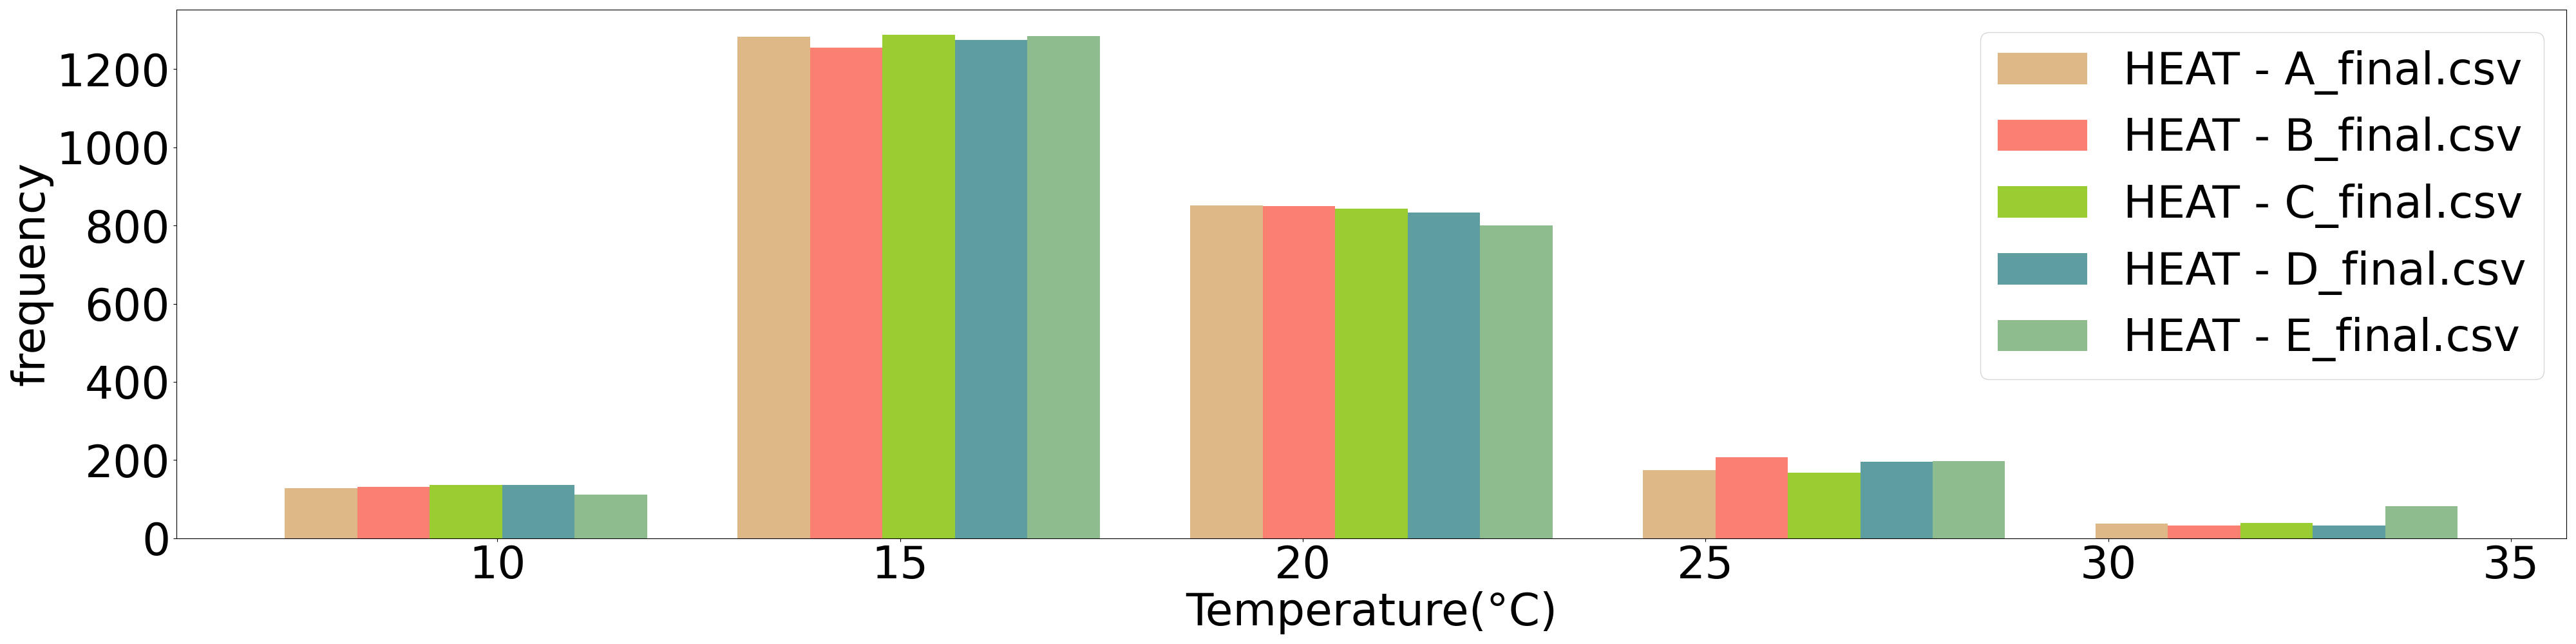
\includegraphics[width=0.8\textwidth]{images/multi_hist_bar_05.png} 
\caption{Frequency statistics of Temperature values of 5 sensors (bar number = 5)}
\end{figure}
\begin{figure}[htbp]
\centering
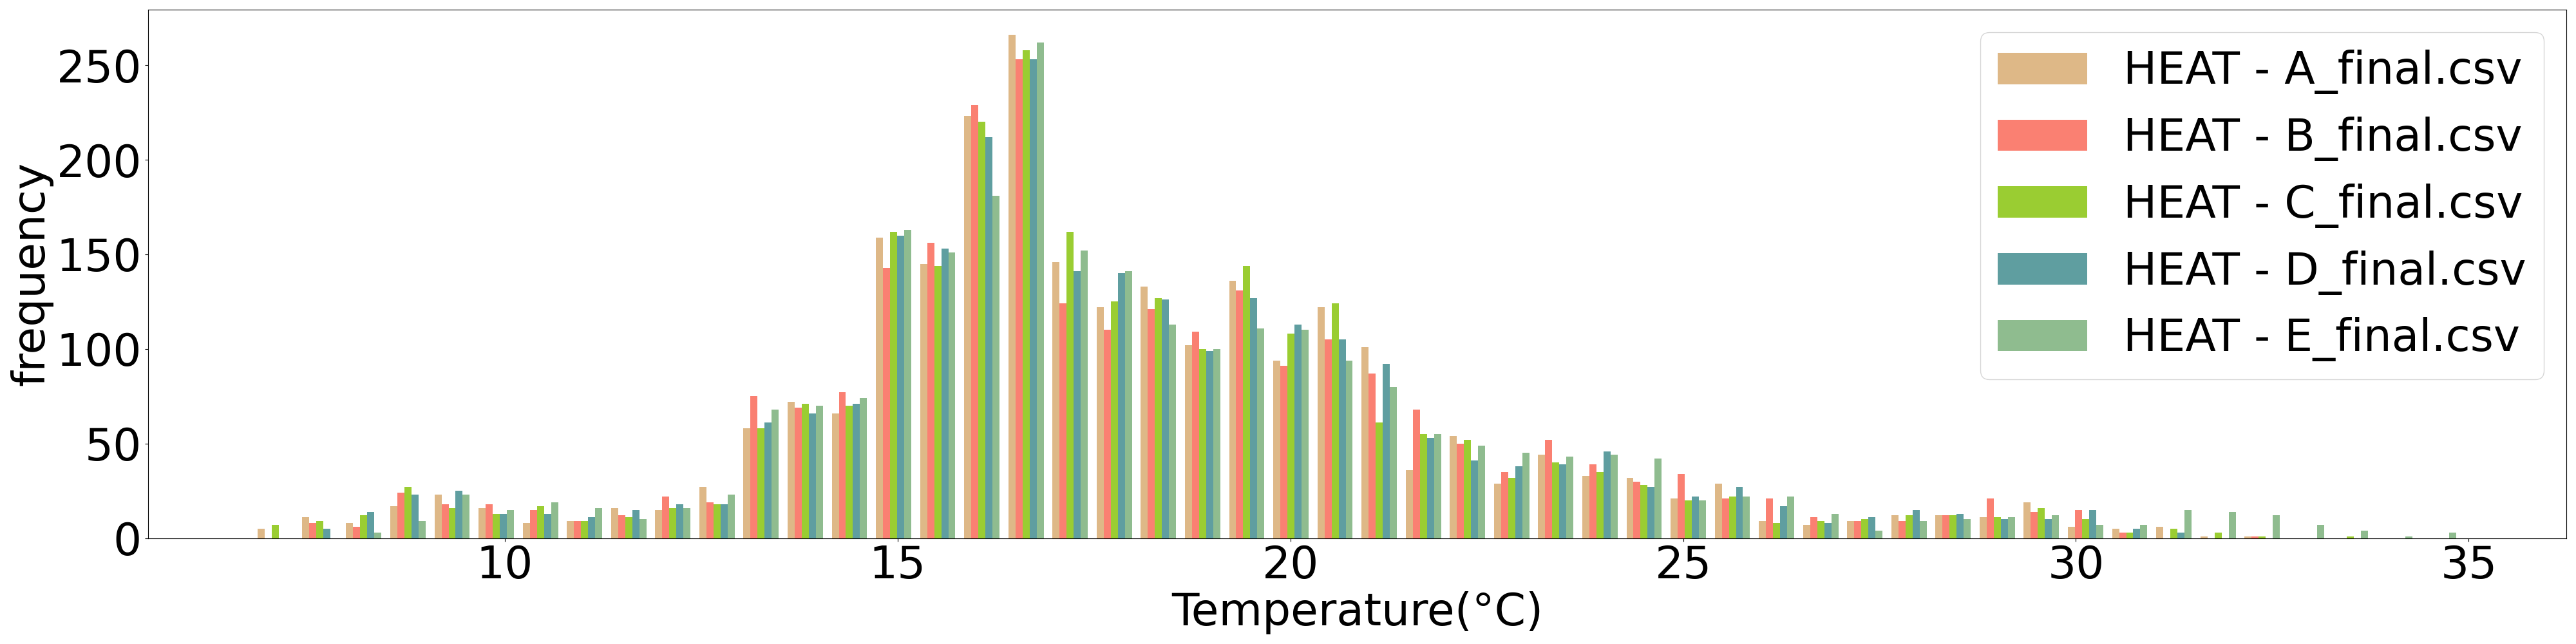
\includegraphics[width=0.8\textwidth]{images/multi_hist_bar_50.png} 
\caption{Frequency statistics of Temperature values of 5 sensors (bar number = 50)}
\label{Fig_mult_hist_temperature_50}
\end{figure}

\noindent Compared to \textbf{Figure 1}, \textbf{Figure 2} can show more details of the distribution. For example, when \textbf{Temperatures} is between 13°C and 15°C, the statistics are relatively stable. And after the frequency of \textbf{Temperature} value reaching the maximum value, the statistical value drops sharply. These details are missing in \textbf{Figure 1}. That why it is very important to choose a appropriate bar number.

\subsection{Question A1.3}
\begin{figure}[htbp]
\centering
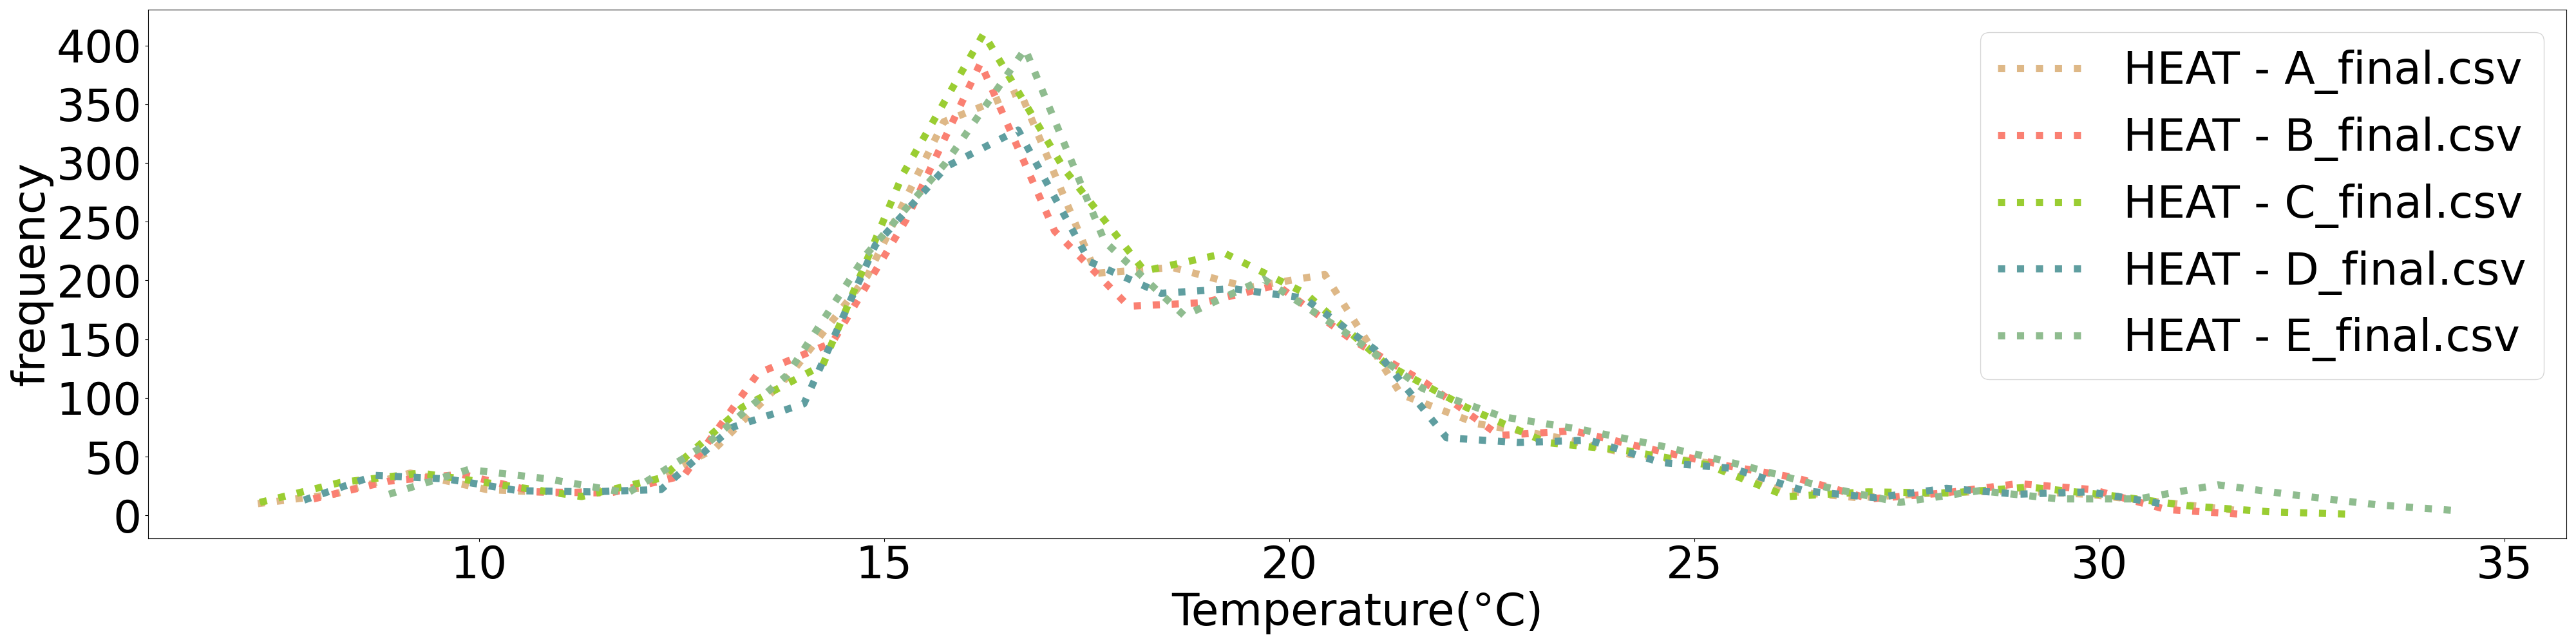
\includegraphics[width=0.8\textwidth]{images/freq_polygen_temp.png} 
\caption{Frequency polygons of Temperature values of 5 sensors}
\label{Fig_mult_hist_temperature_05}
\end{figure}
\newpage
\subsection{Question A1.4}
\begin{figure}[htbp]
\centering
\subfigure[temperature]{
\begin{minipage}[t]{0.33\linewidth}
\centering
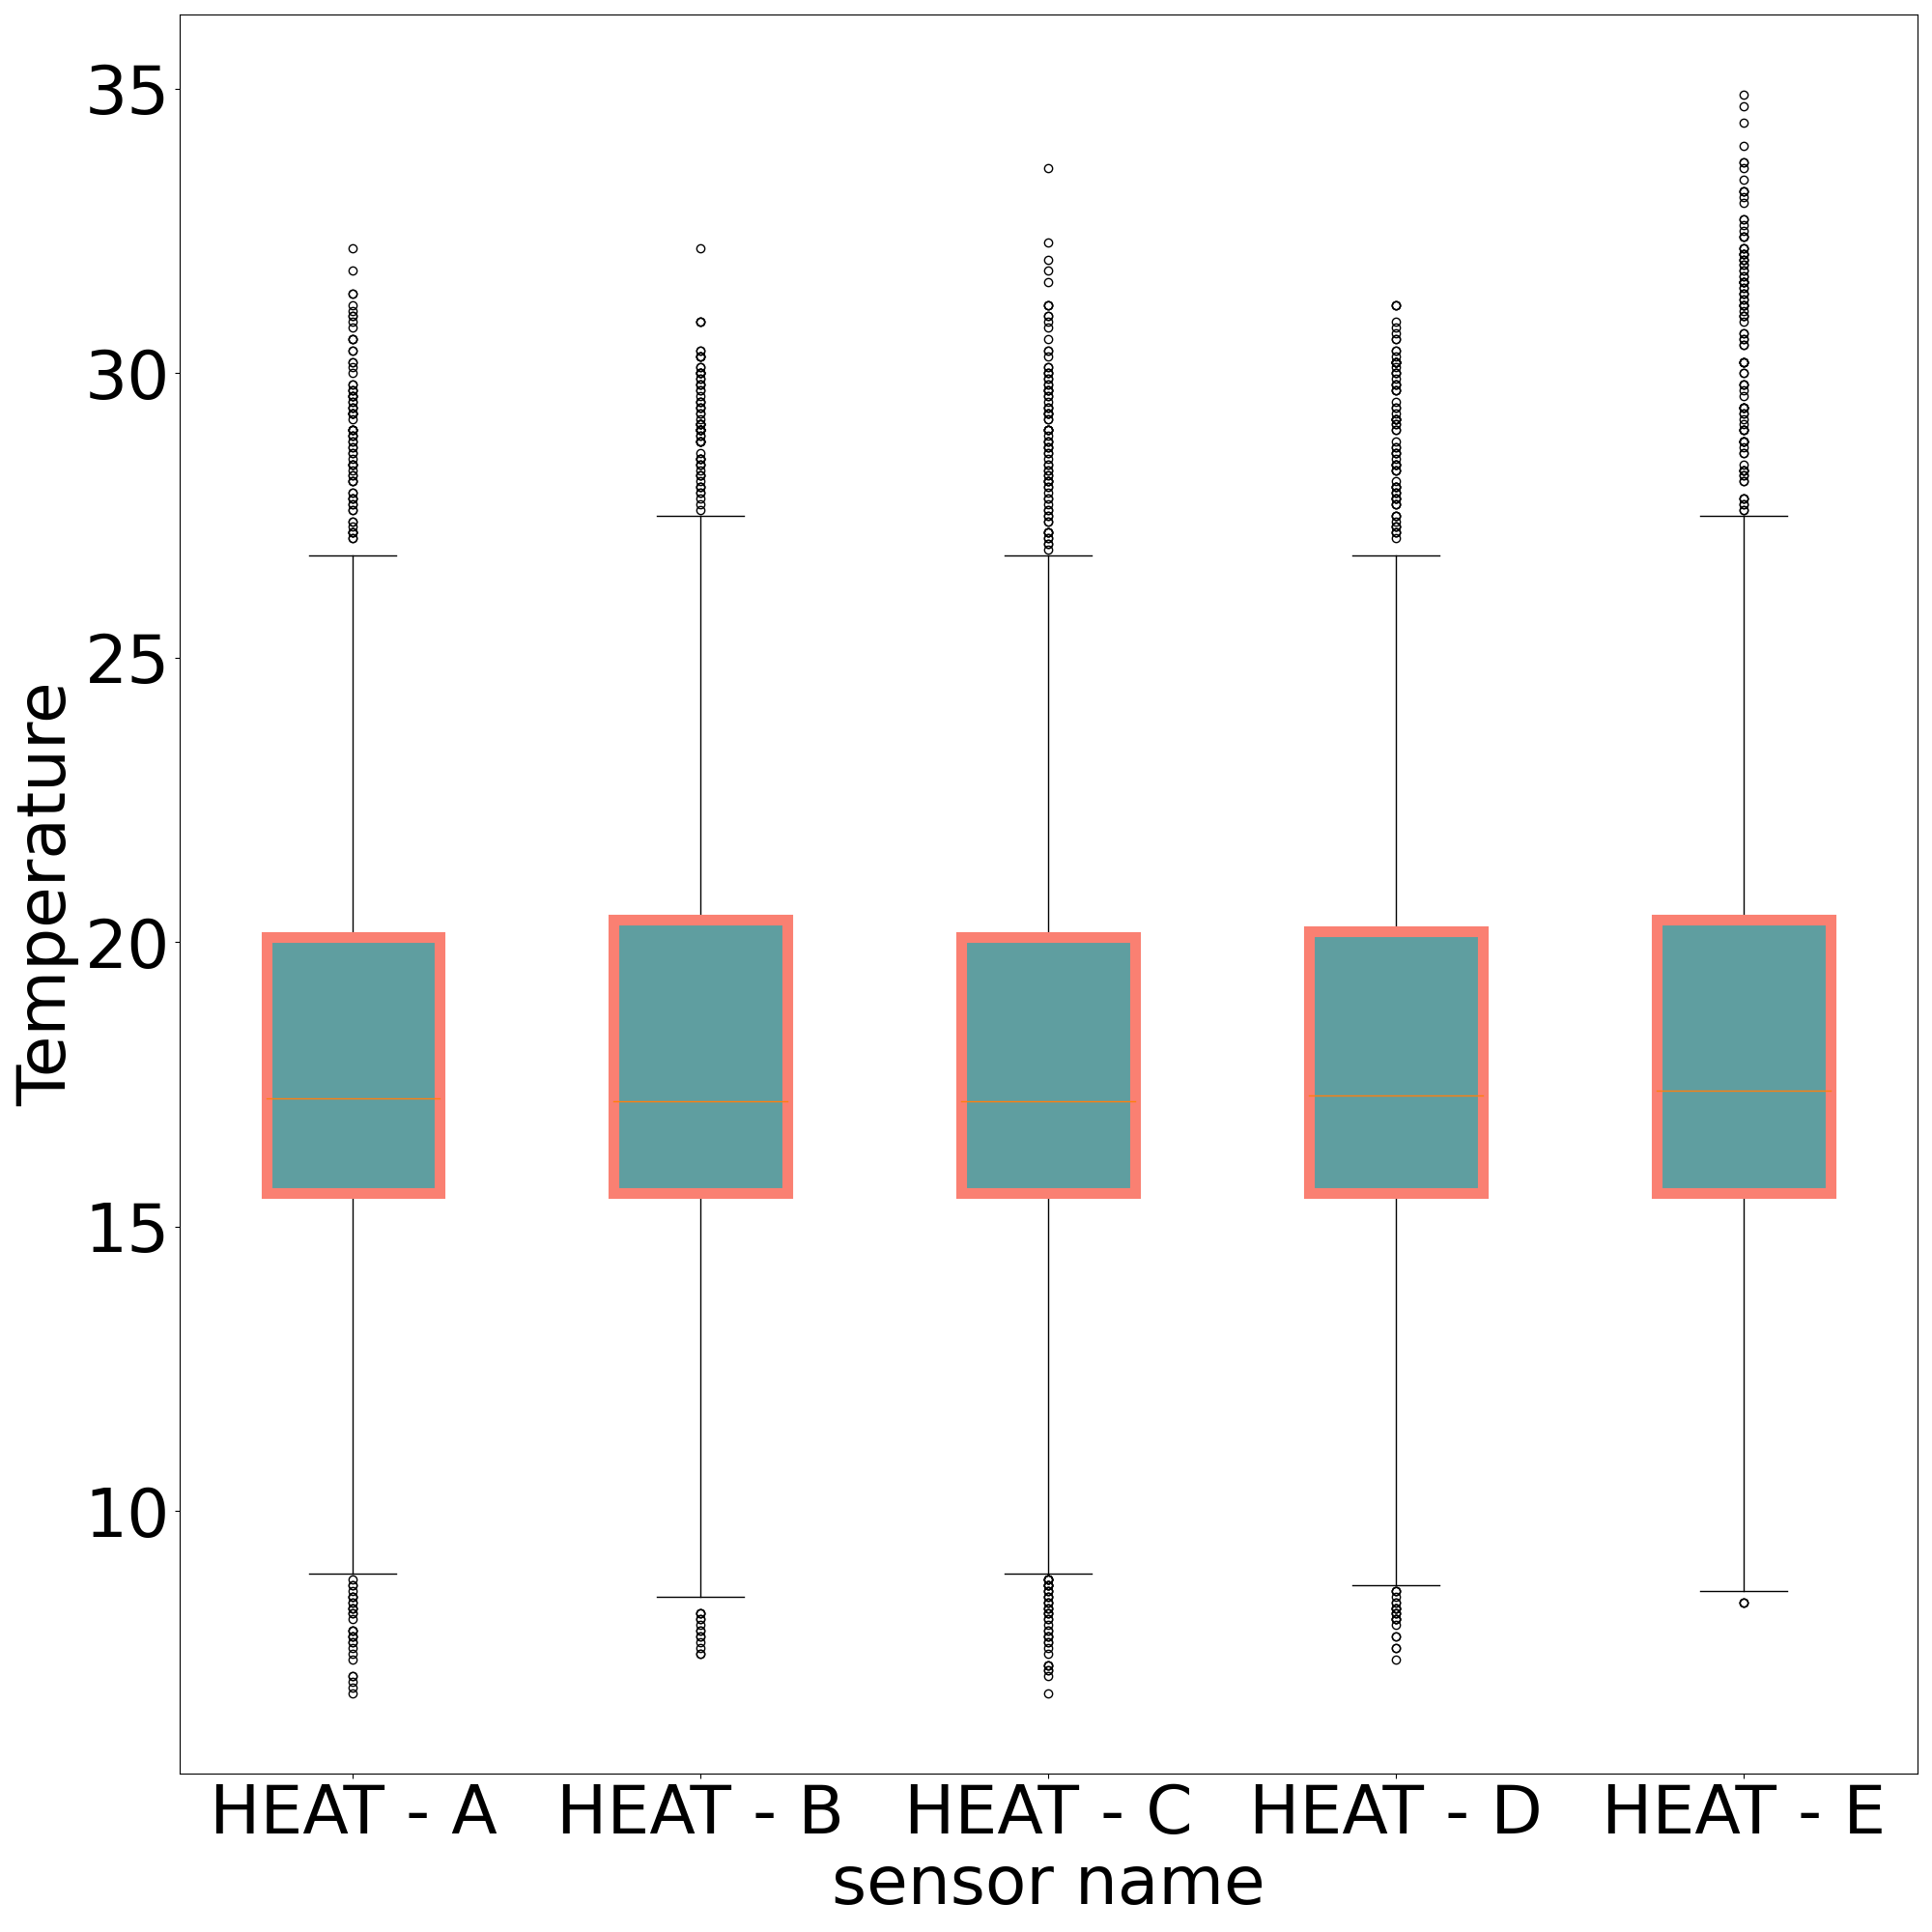
\includegraphics[scale=0.065]{images/boxplot_temp.png}
\end{minipage}
}%
\subfigure[wind speed]{
\begin{minipage}[t]{0.33\linewidth}
\centering
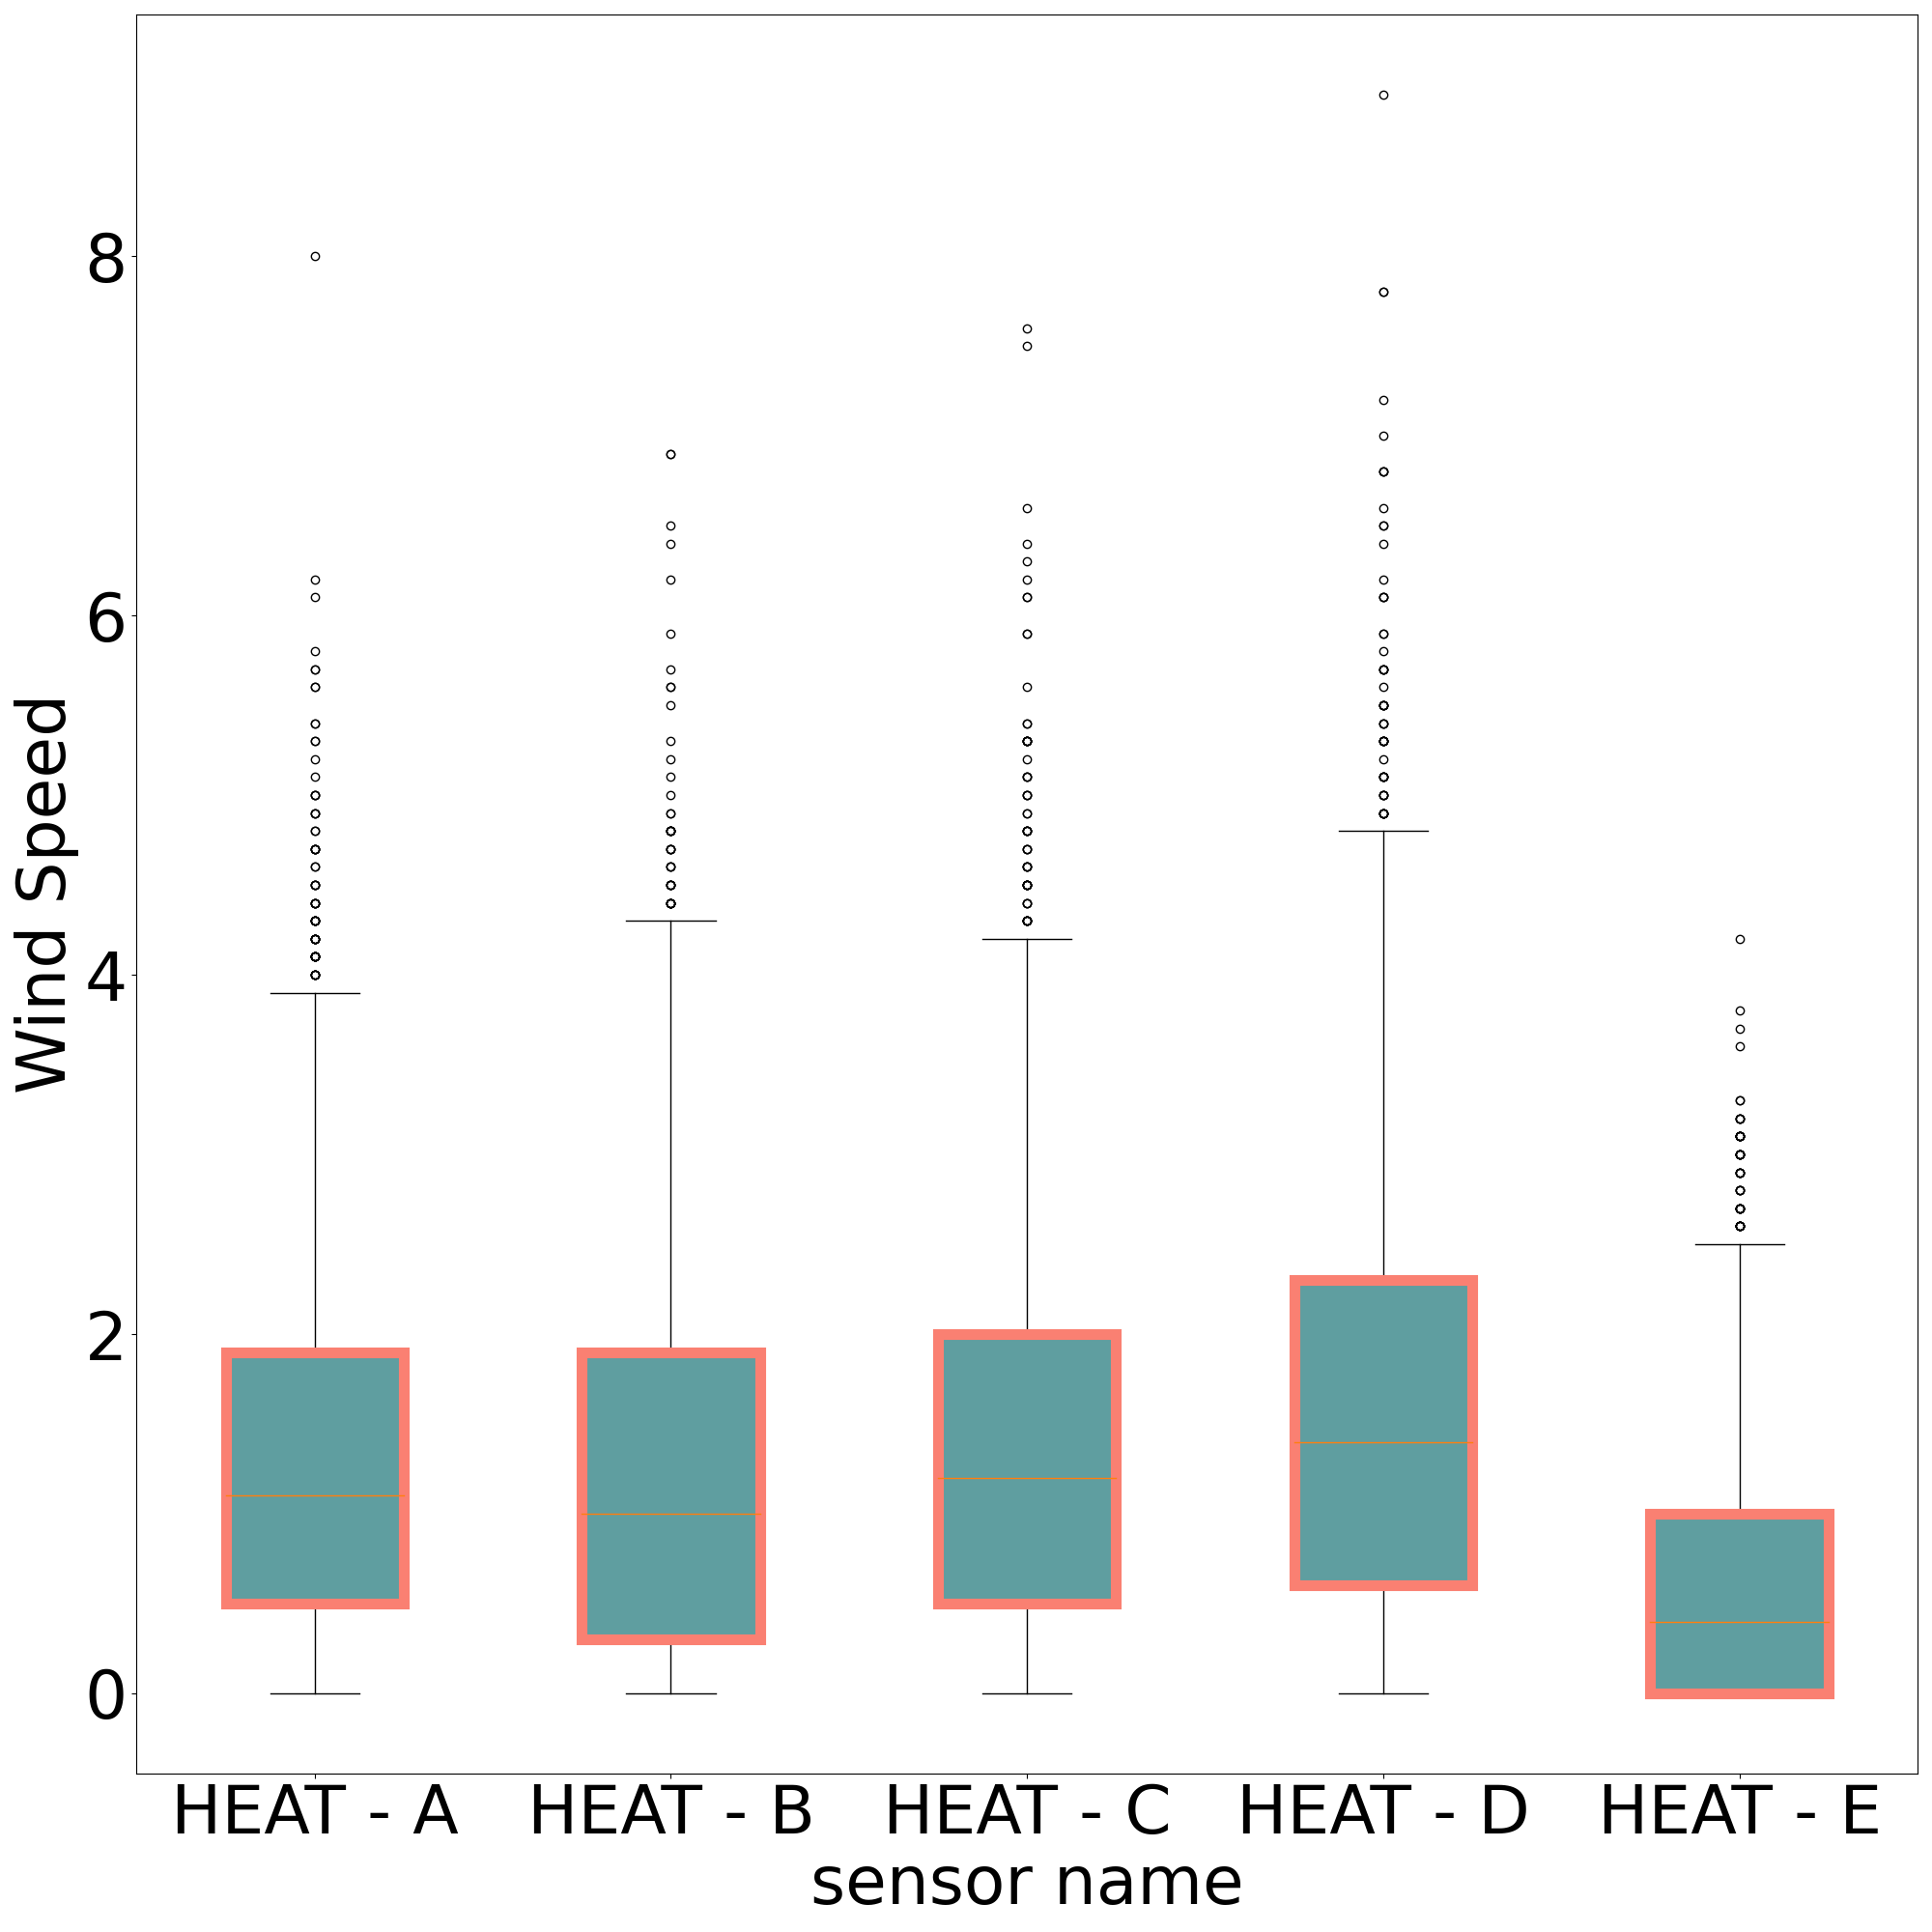
\includegraphics[scale=0.065]{images/boxplot_WS.png}
\end{minipage}%S
}%
\subfigure[wind direction]{
\begin{minipage}[t]{0.33\linewidth}
\centering
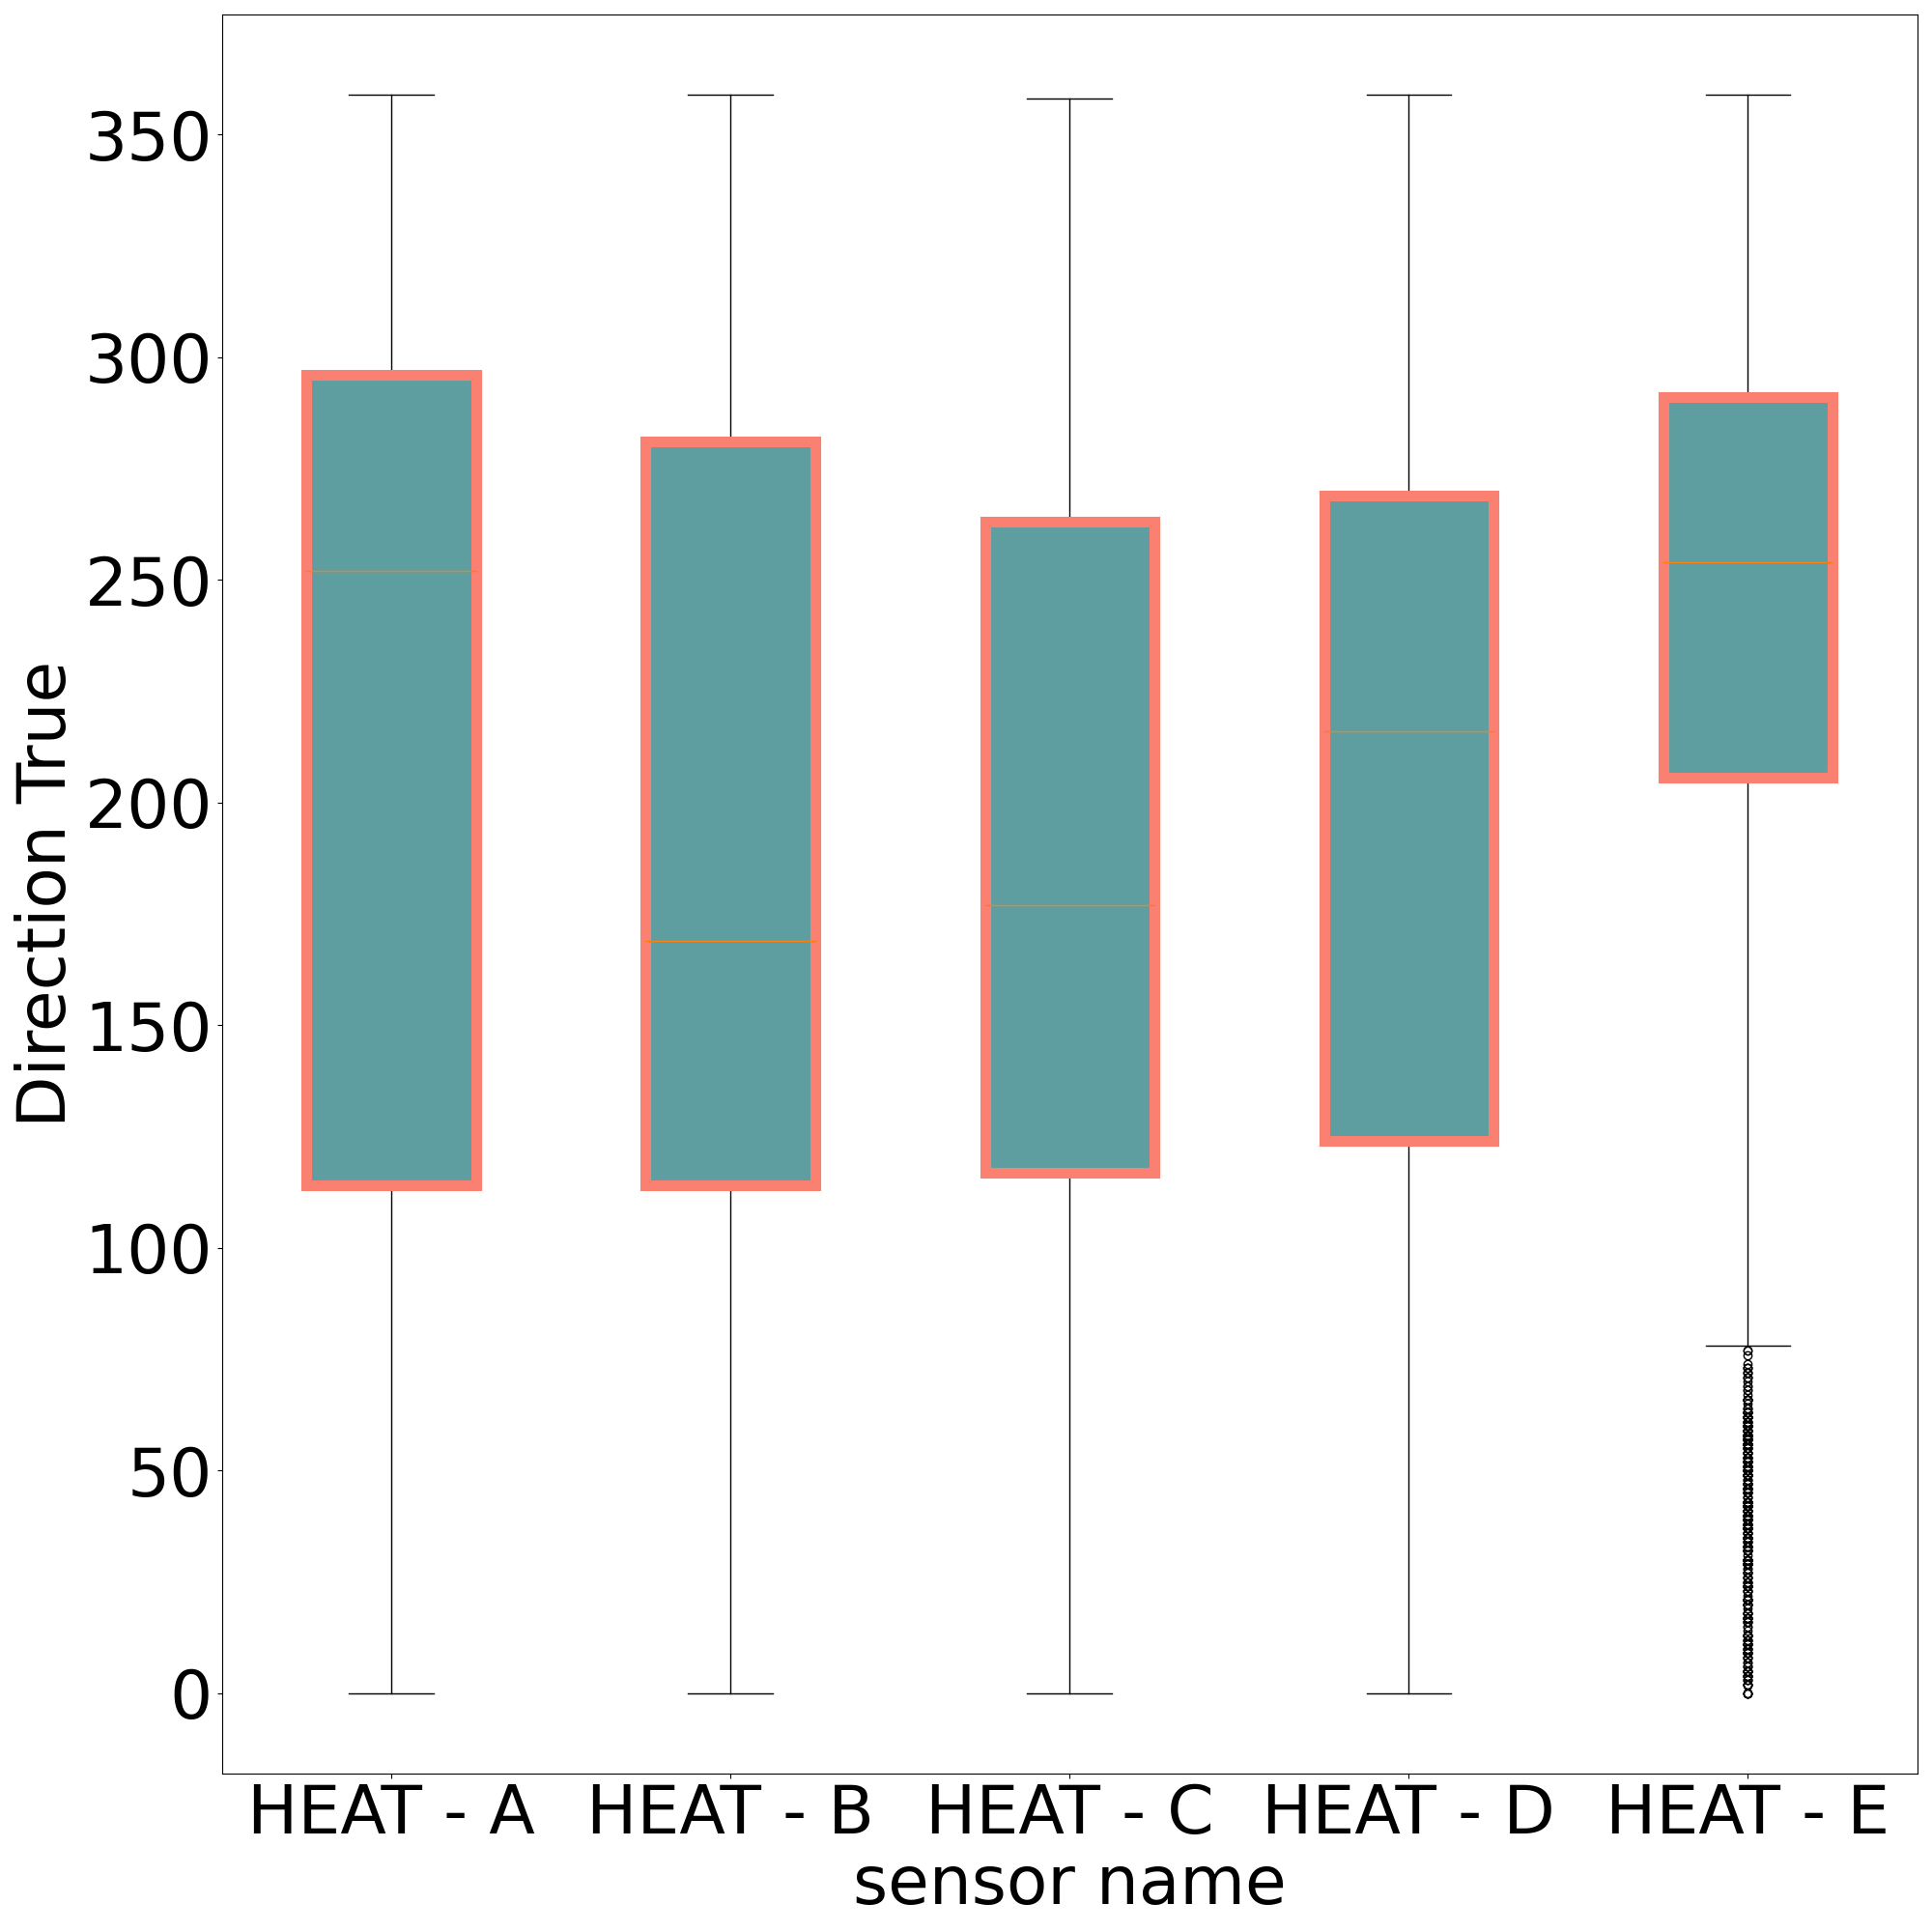
\includegraphics[scale=0.065]{images/boxplot_WD.png}
\end{minipage}
}%
\centering
\caption{Boxplot of Temperature, Wind Speed, Wind Direction values of 5 sensors}
\end{figure}

\section{Exercises after Lecture A2}
\subsection{Question A2.1}

In order to strike a balance between information and readability (especially for \textbf{Figure 5 (a)}), the \textbf{Rice Rule} is used to determine the number of bars.

\begin{figure}[htbp]
\centering
\subfigure[PMF]{
\begin{minipage}[t]{0.33\linewidth}
\centering
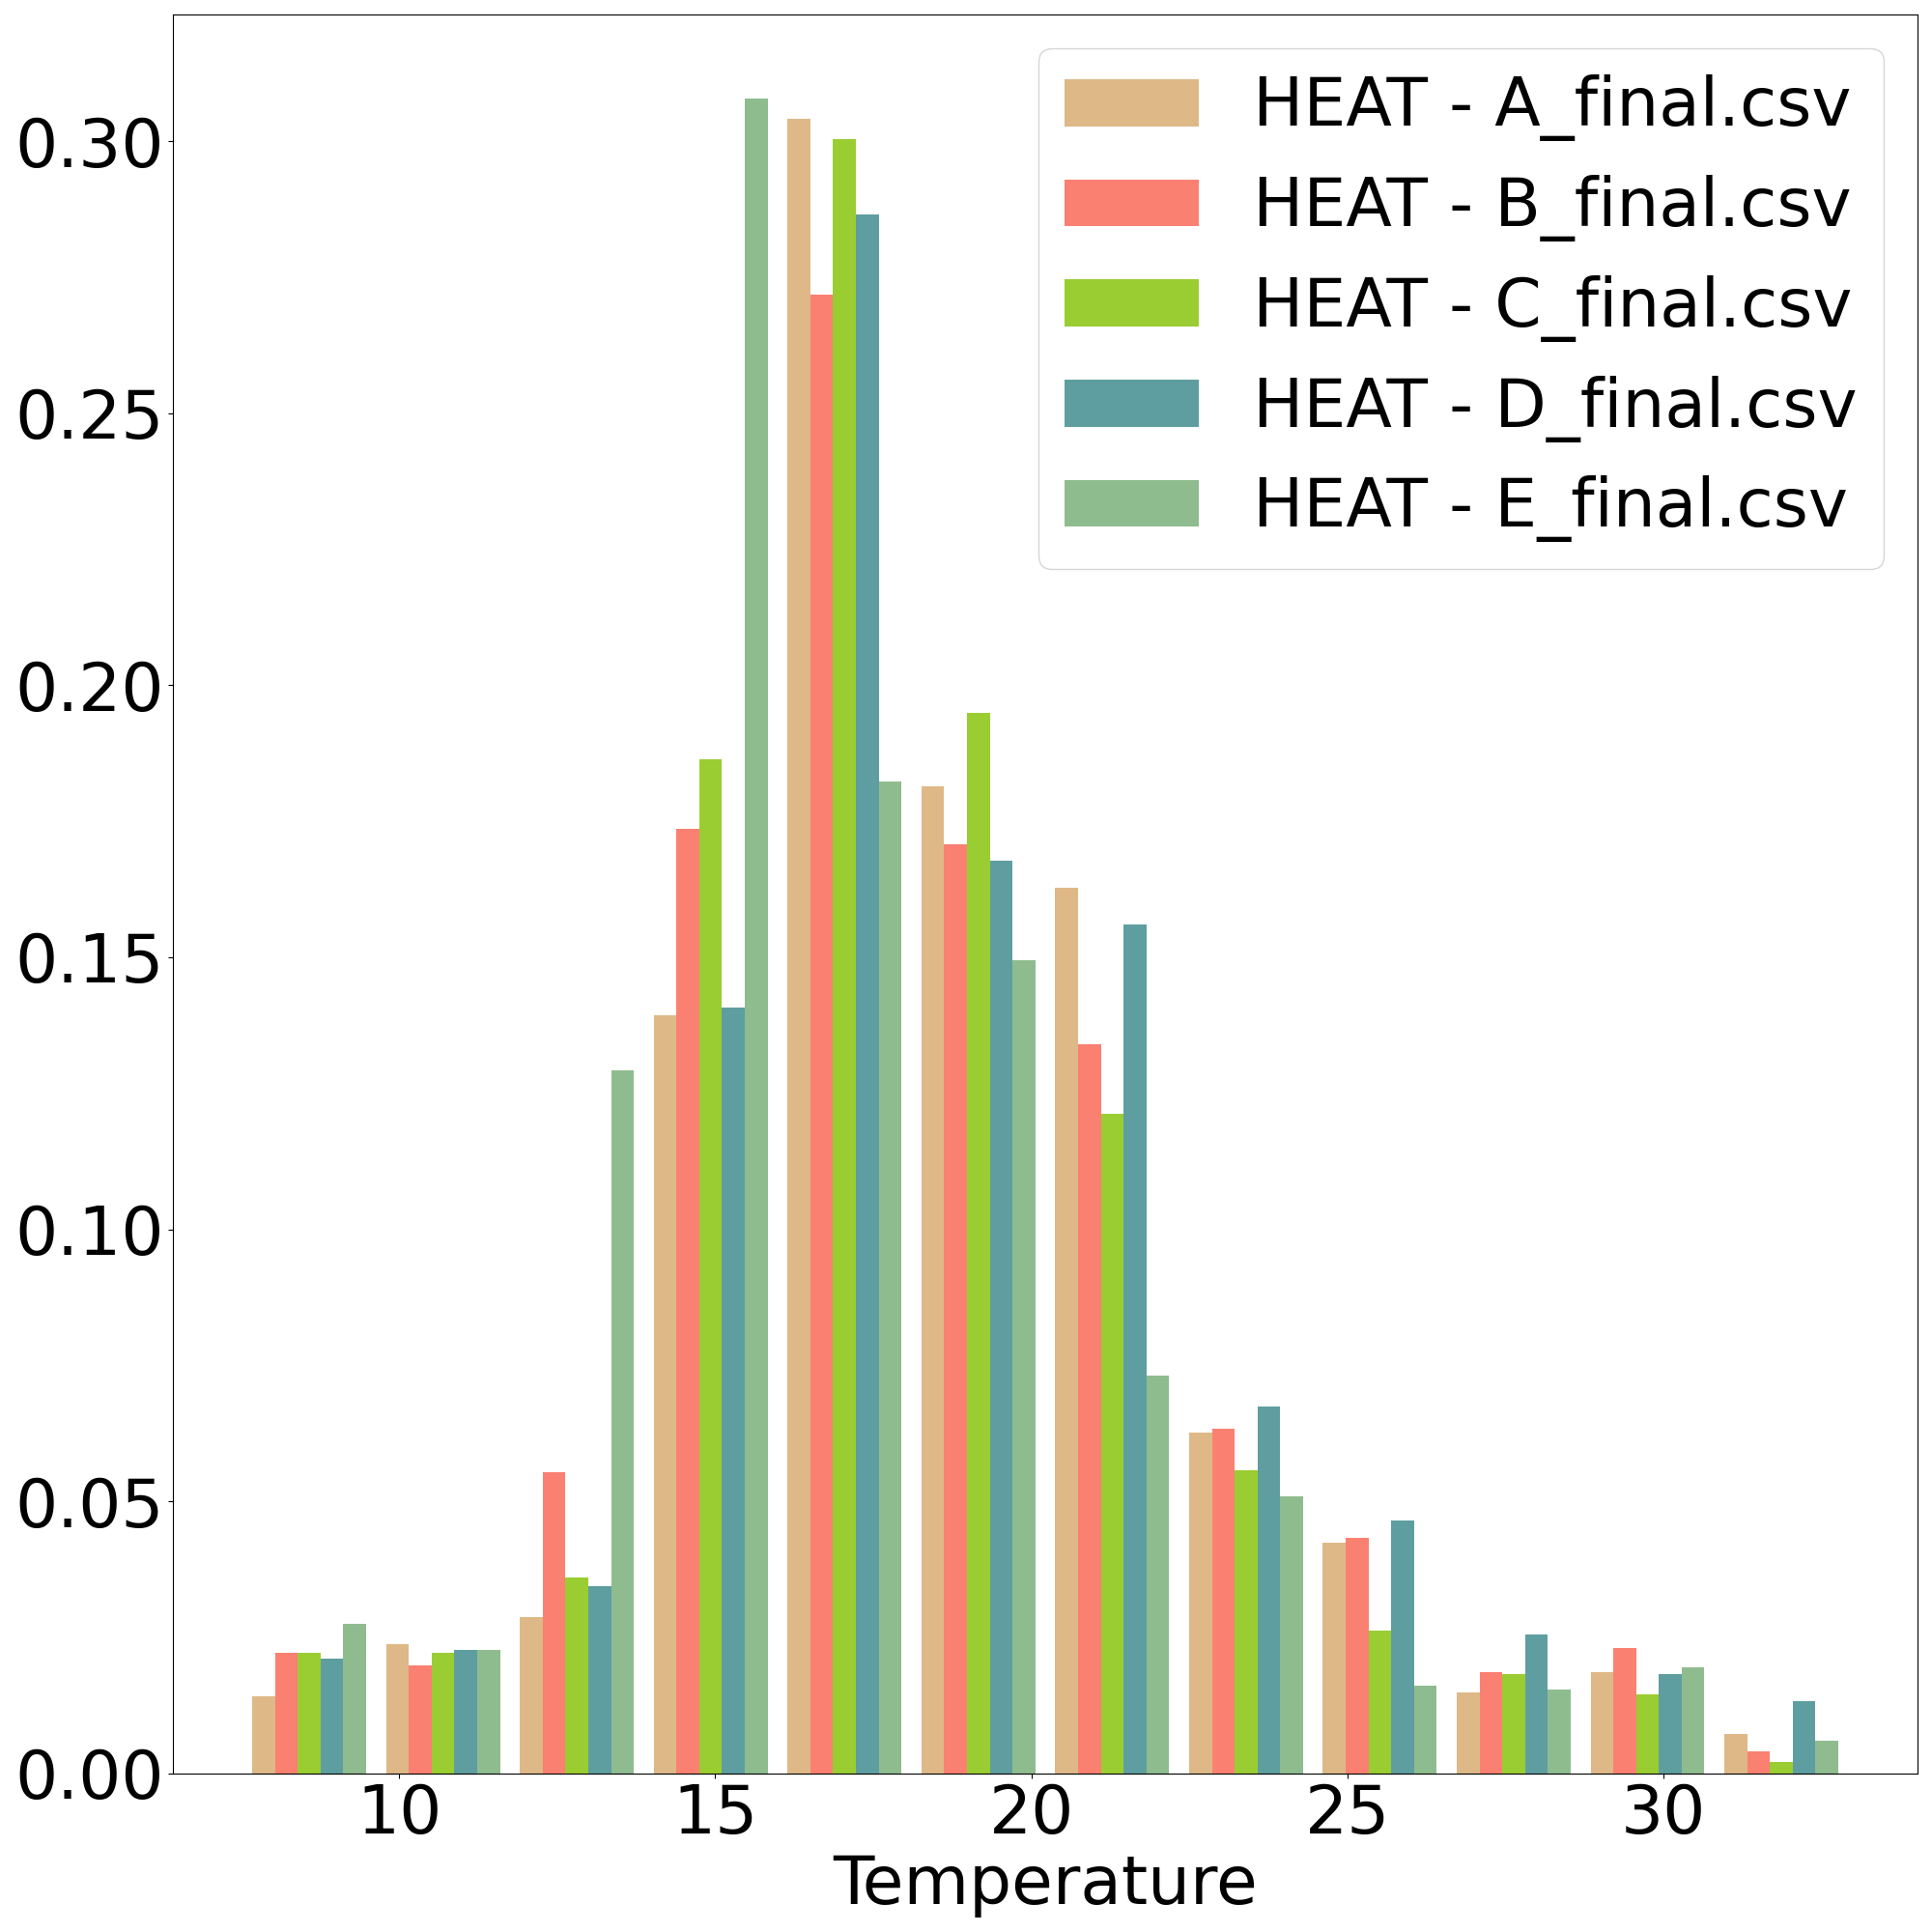
\includegraphics[scale=0.065]{images/pmf_temp.png}
\end{minipage}
}%
\subfigure[PDF]{
\begin{minipage}[t]{0.33\linewidth}
\centering
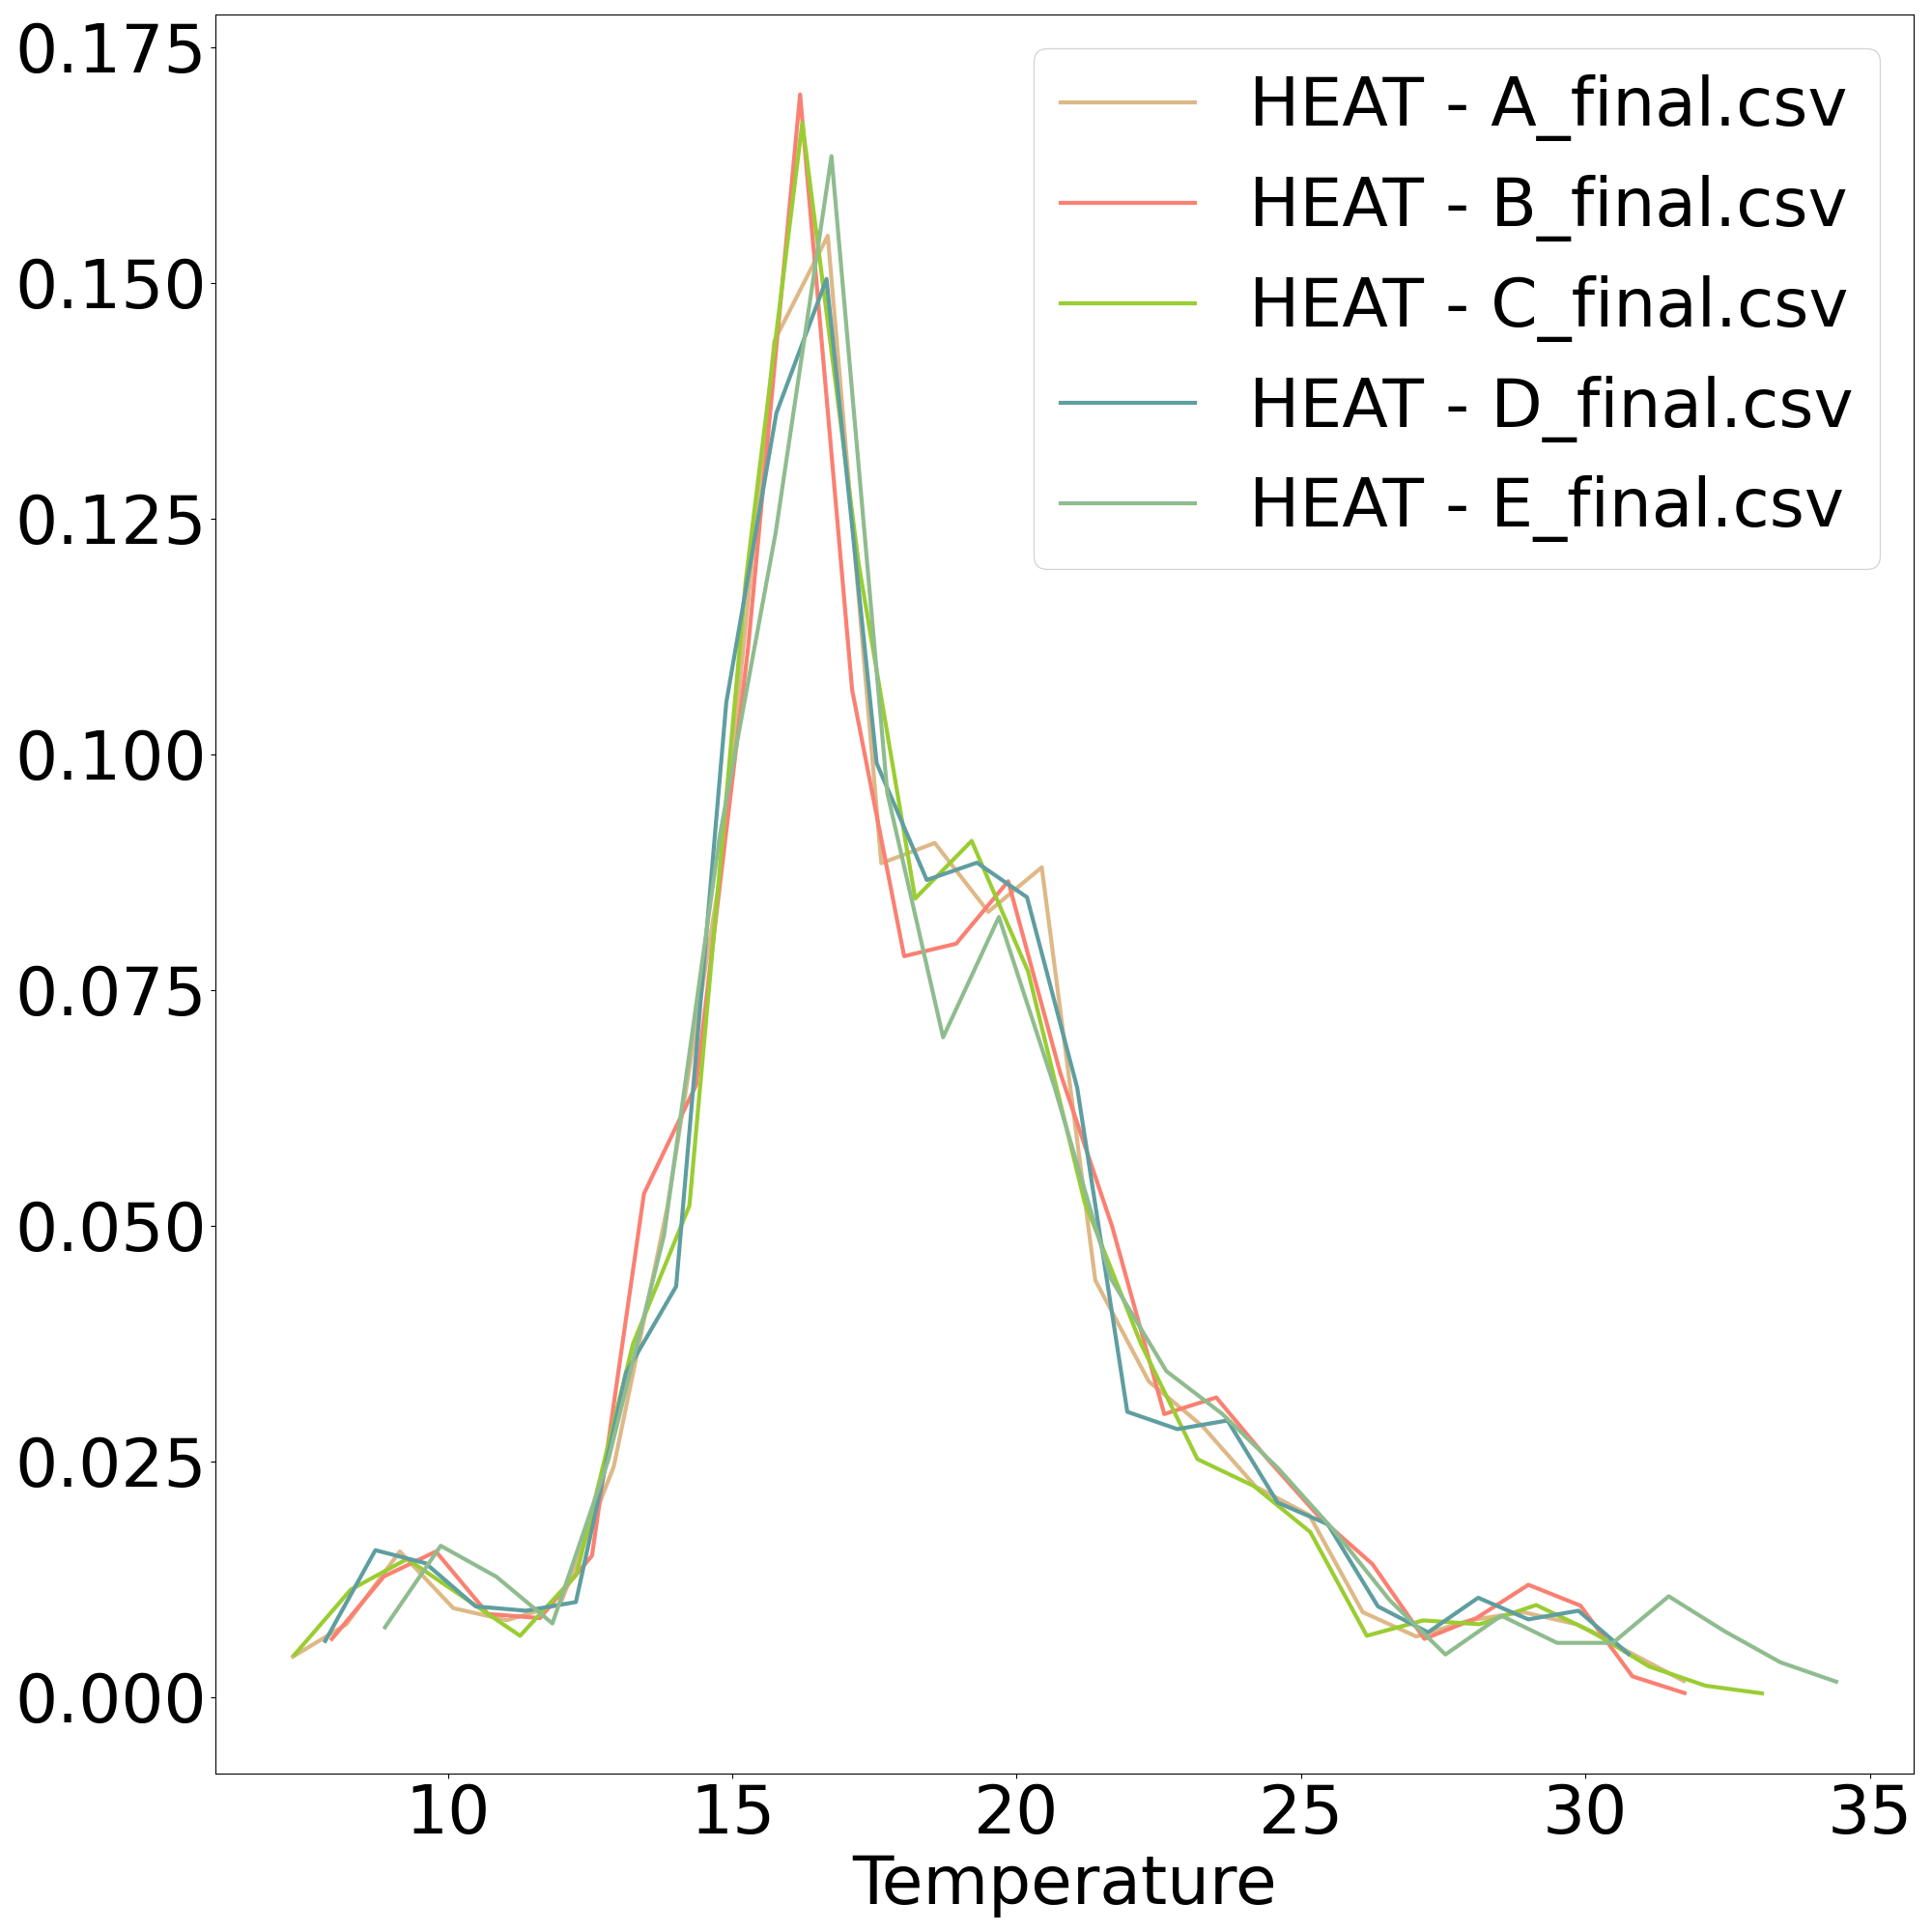
\includegraphics[scale=0.065]{images/pdf_temp.png}
\end{minipage}%S
}%
\subfigure[CDF]{
\begin{minipage}[t]{0.33\linewidth}
\centering
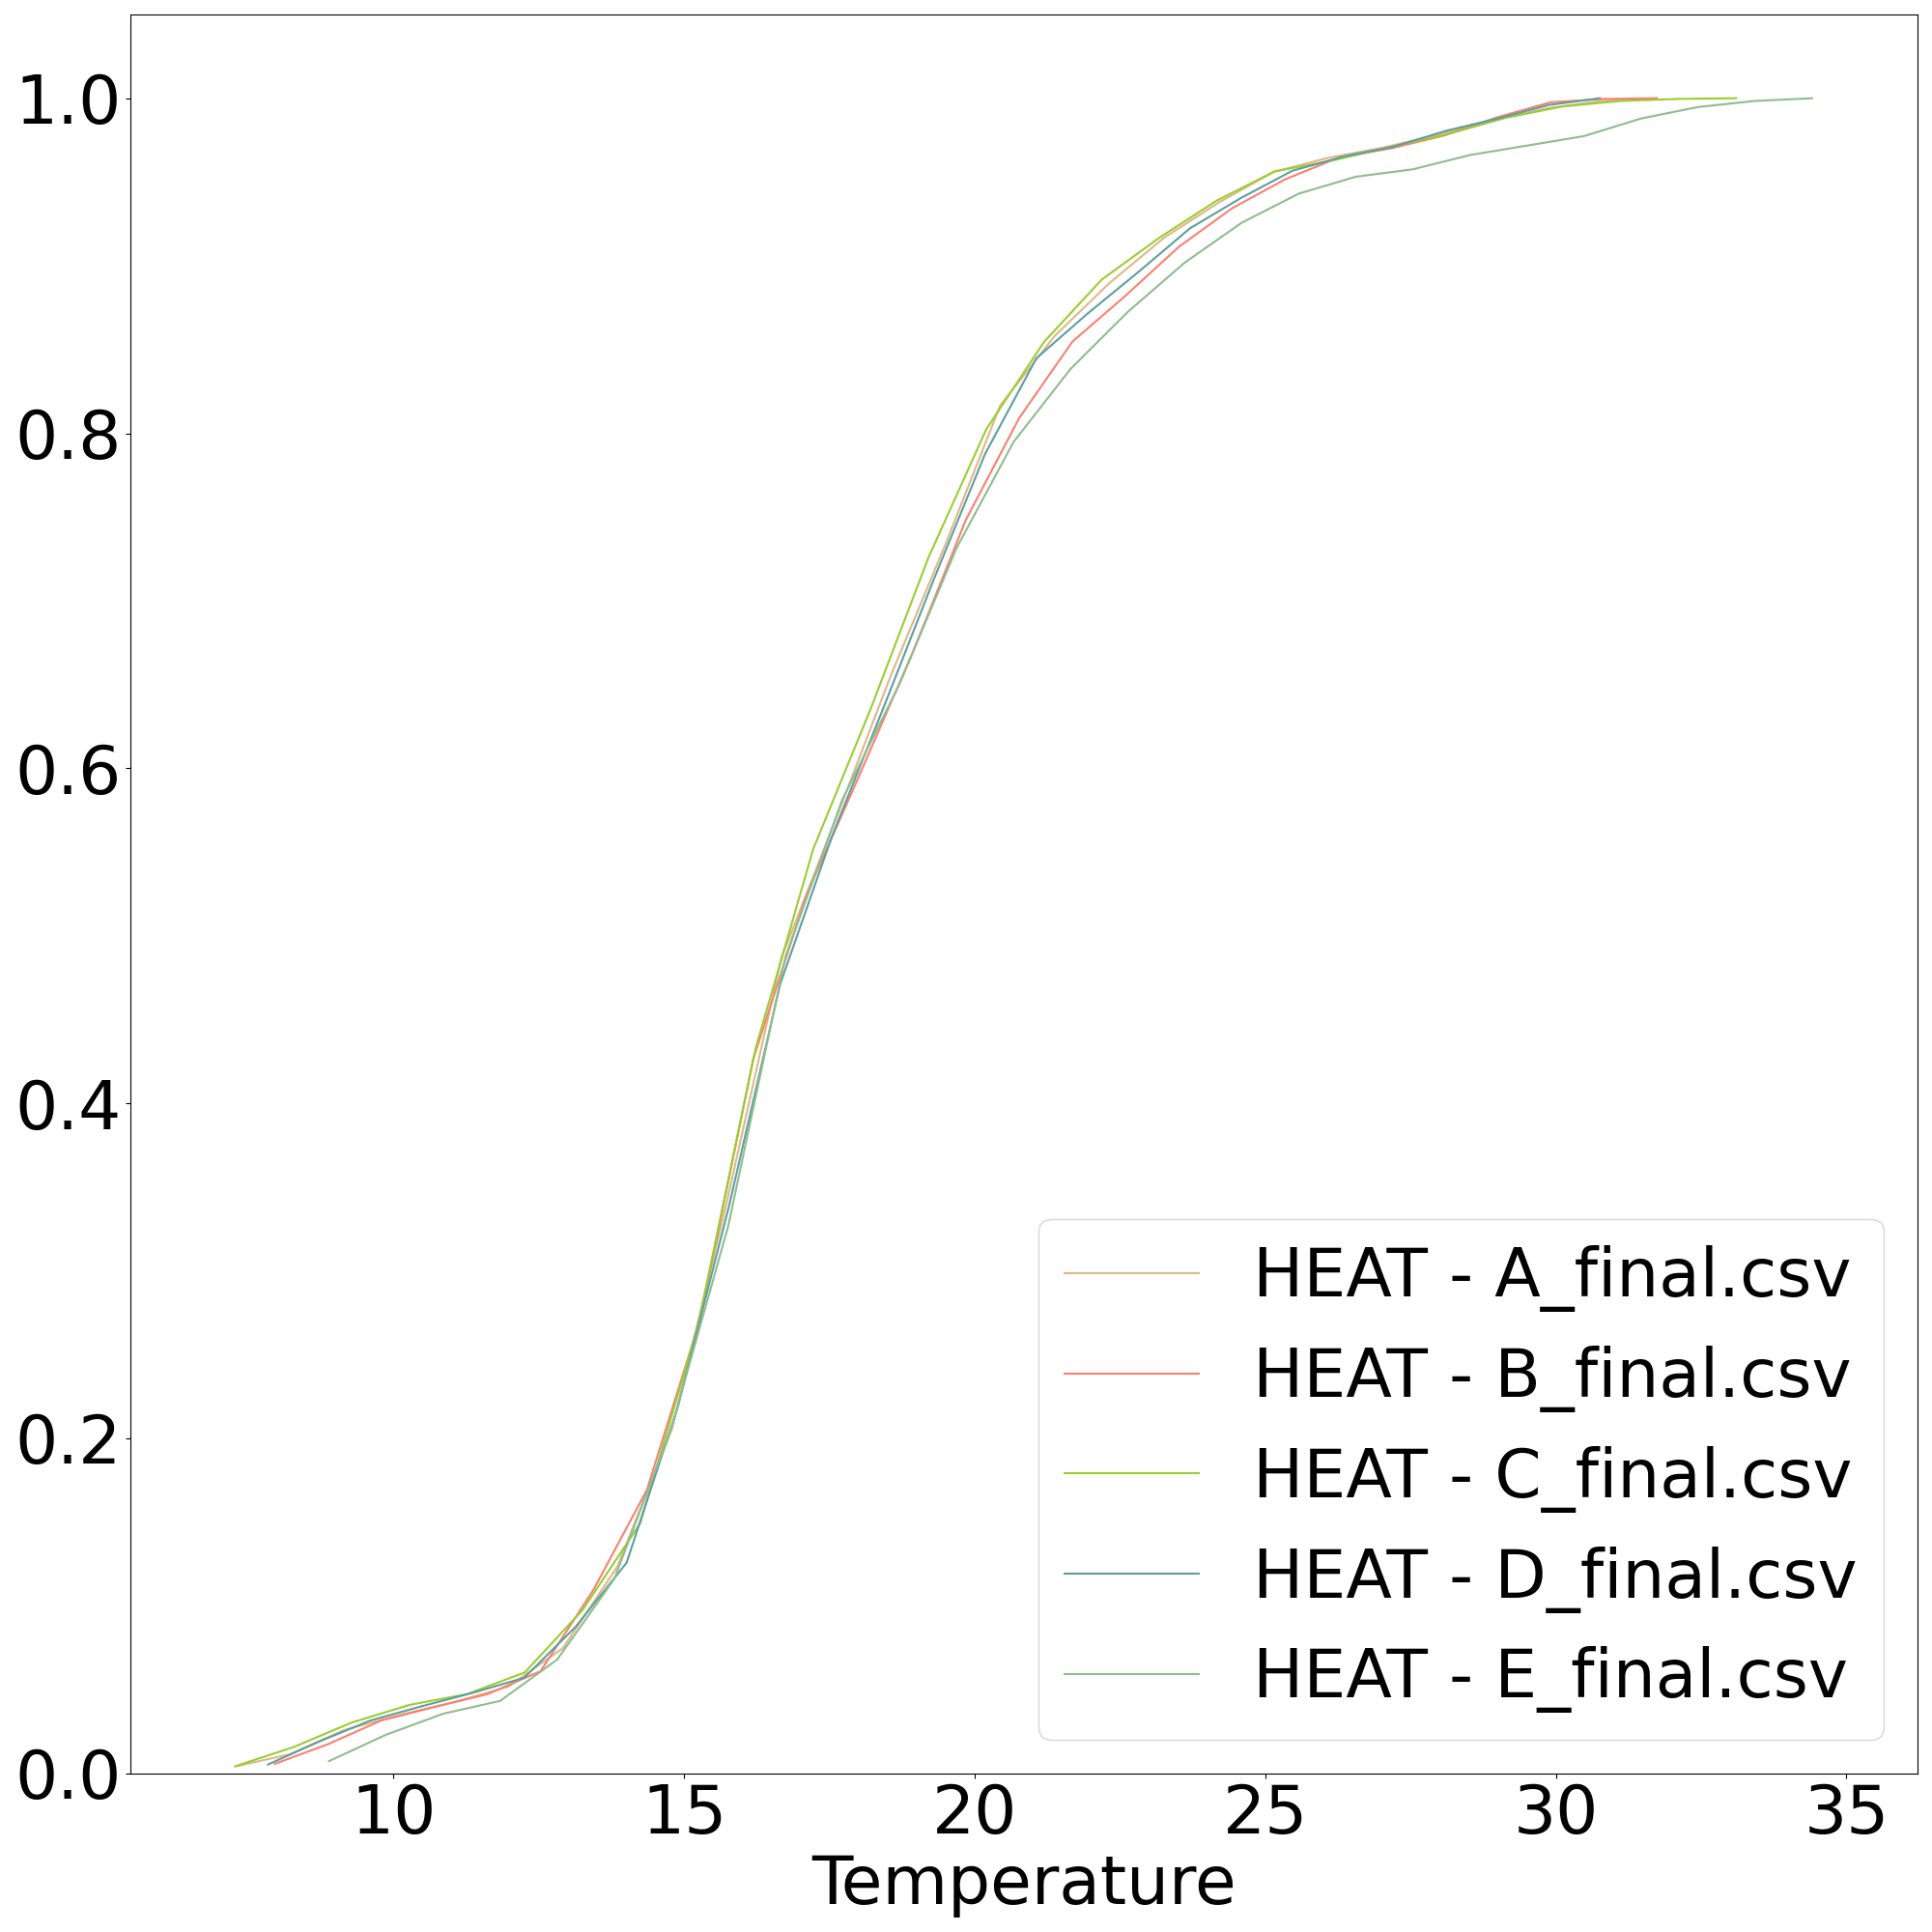
\includegraphics[scale=0.065]{images/cdf_temp.png}
\end{minipage}
}%
\centering
\caption{PMF, PDF and CDF of Temperature values of 5 sensors}
\end{figure}
\noindent The PMF images of 5 sensors show the following information:
\begin{itemize}
    \item The 5 PMF images are similar in general.
    \item All PMF images are positive skewness.
    \item The left tails of these 5 PMF images are shorter than the right tails.
    \item The kurtosis rankings of these 5 images are:
    
    \textbf{sensor E}>\textbf{sensor A}>\textbf{sensor C}>\textbf{sensor D}>\textbf{sensor B}.
    \item The positive skewness of \textbf{sensor E} is more obvious than others. Its trends of growth and decline both are also more dramatic.
\end{itemize}

\noindent The PDF images of 5 sensors show the following information:
\begin{itemize}
    \item The 5 PDF images are also similar in general, especially when temperature value is between 13°C and 15°C.
    \item All PDF images are also positive skewness.
    \item The left tails of these 5 PDF images are shorter than the right tails, too.
    \item The kurtosis rankings of these 5 images are:
    
    \textbf{sensor C}>\textbf{sensor A}>\textbf{sensor D}>\textbf{sensor B}>\textbf{sensor E}.
    \item The left tail of \textbf{sensor E} is shorter than others, while its right tail is much longer.
\end{itemize}

\noindent The CDF images of 5 sensors show the following information:
\begin{itemize}
    \item The 5 CDF images are also similar in general, especially when temperature value is between 13°C and 15°C. This section corresponds to the head section of the PDF. 
    \item The CDF images have distinct differences in the front and rear sections (corresponding to the tail section in the PDF).
    \item When temperature is larger than 20°C, the CDF of \textbf{sensor E} is the lowest. This is consistent with the fact that it falls too fast after reaching its peak in PDF image.
\end{itemize}

\subsection{Question A2.2}
\begin{figure}[htbp]
\centering
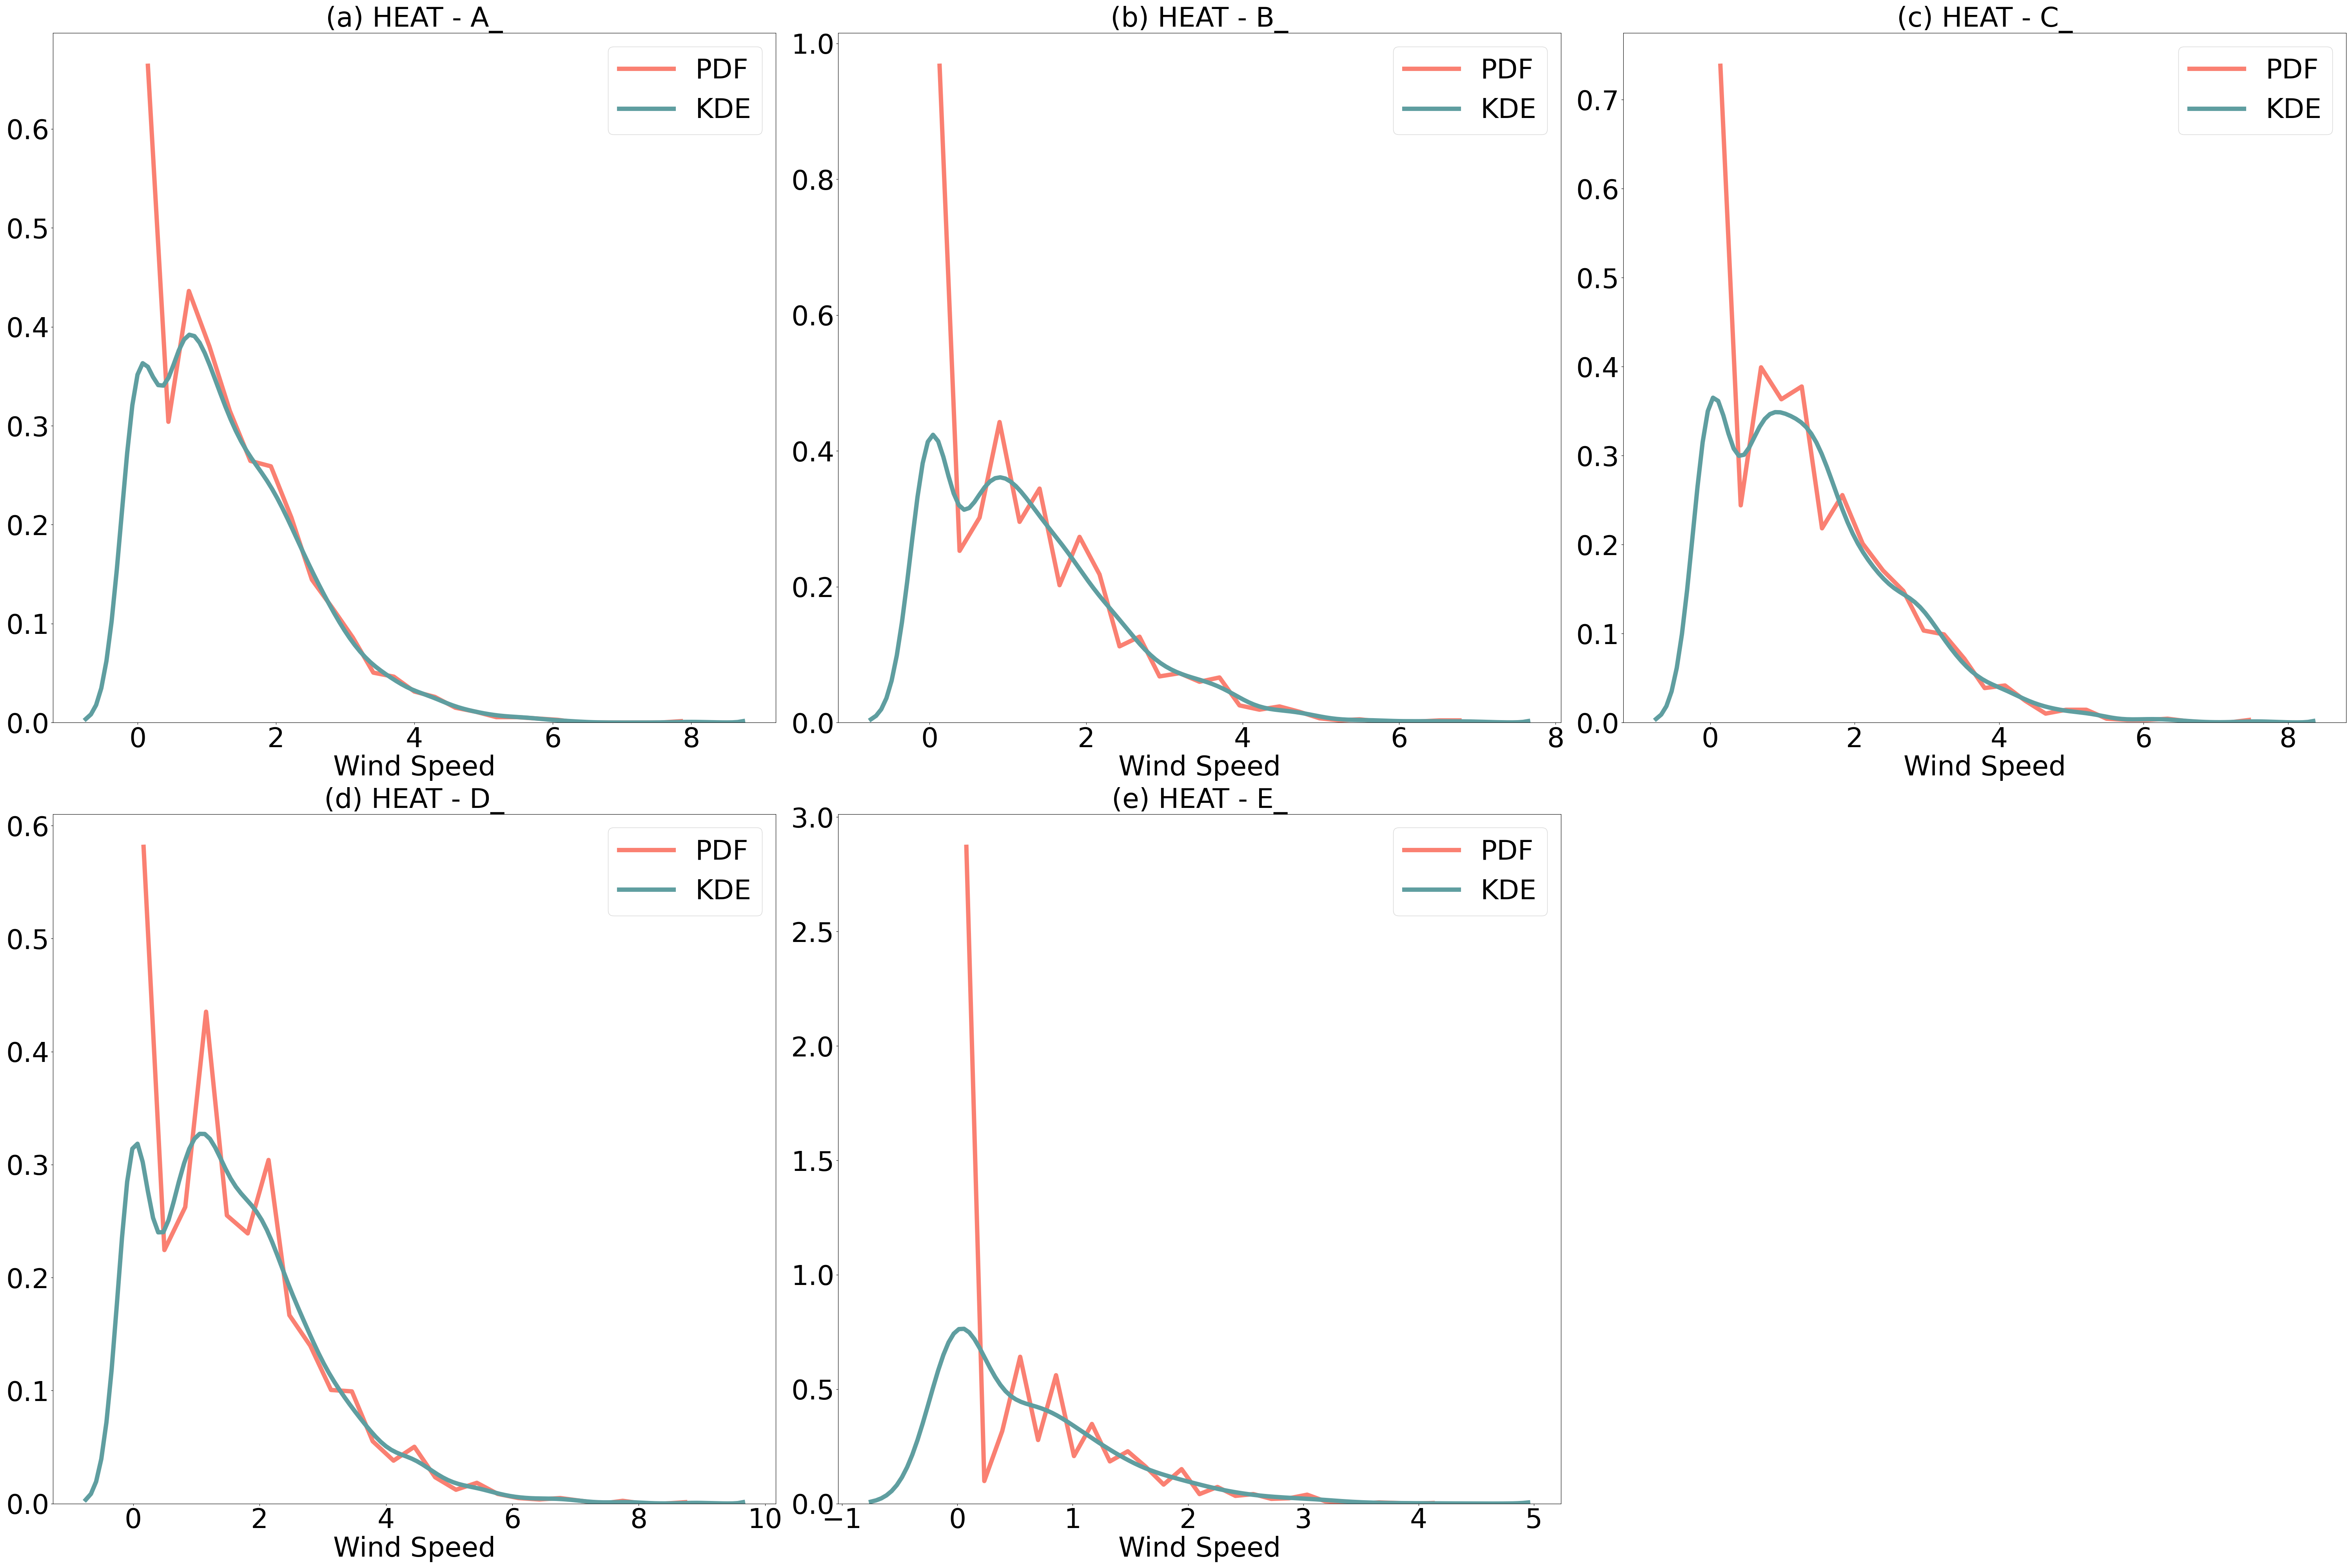
\includegraphics[width=0.7\textwidth]{images/pdf_and_kde_WS.png} 
\caption{PDF and KDE of Wind Speed values of 5 sensors}
\end{figure}

\noindent Comparing the 5 PDF and KDE(bw=0.25) images in \textbf{Figure 6} can get the following differences:
\begin{itemize}
    \item KDE is generally smoother than PDF images.
    \item KDE may lose information about the peaks and troughs of PDF images, especially if the function has a high kurtosis or the image is very volatile. For example, Kde may reverse the relationship between peaks and subpeaks(\textbf{Figure 6 (d)}).
\end{itemize}

\section{Exercises after Lecture A3}
\subsection{Question A3.1}

\begin{table}[htbp]
  \centering
  \caption{Correlations between 5 sensors for the Temperature}
    \begin{tabular}{c|ccccccc|ccccc}
    \multicolumn{1}{c}{} &       &       & (a) Pearson &       &       &       & \multicolumn{1}{c}{} &       &       & (b) Spearmann &       &  \\
    \multicolumn{1}{c}{} &       &       &       &       &       &       & \multicolumn{1}{c}{} &       &       &       &       &  \\
          & A     & B     & C     & D     & E     &       &       & A     & B     & C     & D     & E \\
\cmidrule{1-6}\cmidrule{8-13}    A     & /     & 0.988  & 0.989  & 0.986  & 0.969  &       & A     & /     & 0.987  & 0.988  & 0.985  & 0.972  \\
    B     & 0.988  & /     & 0.984  & 0.986  & 0.972  &       & B     & 0.987  & /     & 0.985  & 0.986  & 0.977  \\
    C     & 0.989  & 0.984  & /     & 0.989  & 0.972  &       & C     & 0.988  & 0.985  & /     & 0.988  & 0.977  \\
    D     & 0.986  & 0.986  & 0.989  & /     & 0.971  &       & D     & 0.985  & 0.986  & 0.988  & /     & 0.976  \\
    E     & 0.969  & 0.972  & 0.972  & 0.971  & /     &       & E     & 0.972  & 0.977  & 0.977  & 0.976  & / \\
    \end{tabular}%
\end{table}%

\begin{table}[htbp]
  \centering
  \caption{Correlations between 5 sensors for the Wet Bulb Globe Temperature (WBGT)}
    \begin{tabular}{c|ccccccc|ccccc}
    \multicolumn{1}{c}{} &       &       & (a) Pearson &       &       &       & \multicolumn{1}{c}{} &       &       & (b) Spearmann &       &  \\
    \multicolumn{1}{c}{} &       &       &       &       &       &       & \multicolumn{1}{c}{} &       &       &       &       &  \\
          & A     & B     & C     & D     & E     &       &       & A     & B     & C     & D     & E \\
\cmidrule{1-6}\cmidrule{8-13}    A     & /     & 0.991  & 0.992  & 0.987  & 0.950  &       & A     & /     & 0.992  & 0.992  & 0.988  & 0.949  \\
    B     & 0.991  & /     & 0.990  & 0.988  & 0.954  &       & B     & 0.992  & /     & 0.990  & 0.987  & 0.957  \\
    C     & 0.992  & 0.990  & /     & 0.992  & 0.949  &       & C     & 0.992  & 0.990  & /     & 0.991  & 0.949  \\
    D     & 0.987  & 0.988  & 0.992  & /     & 0.948  &       & D     & 0.988  & 0.987  & 0.991  & /     & 0.949  \\
    E     & 0.950  & 0.954  & 0.949  & 0.948  & /     &       & E     & 0.949  & 0.957  & 0.949  & 0.949  & / \\
    \end{tabular}%
\end{table}%

\begin{table}[htbp]
  \centering
  \caption{Correlations between 5 sensors for the Crosswind Speed}
    \begin{tabular}{l|rrrrccl|rrrrc}
    \multicolumn{1}{c}{} &       &       & \multicolumn{1}{c}{(a) Pearson} &       &       &       & \multicolumn{1}{c}{} &       &       & \multicolumn{1}{c}{(b) Spearmann} &       &  \\
    \multicolumn{1}{c}{} &       &       &       &       &       &       & \multicolumn{1}{c}{} &       &       &       &       &  \\
          & \multicolumn{1}{c}{A} & \multicolumn{1}{c}{B} & \multicolumn{1}{c}{C} & \multicolumn{1}{c}{D} & E     &       &       & \multicolumn{1}{c}{A} & \multicolumn{1}{c}{B} & \multicolumn{1}{c}{C} & \multicolumn{1}{c}{D} & E \\
\cmidrule{1-6}\cmidrule{8-13}    A     & \multicolumn{1}{c}{/} & 0.550  & 0.514  & 0.490  & \multicolumn{1}{r}{0.465 } &       & A     & \multicolumn{1}{c}{/} & 0.597  & 0.577  & 0.602  & \multicolumn{1}{r}{0.538 } \\
    B     & 0.550  & \multicolumn{1}{c}{/} & 0.516  & 0.488  & \multicolumn{1}{r}{0.392 } &       & B     & 0.597  & \multicolumn{1}{c}{/} & 0.591  & 0.605  & \multicolumn{1}{r}{0.500 } \\
    C     & 0.514  & 0.516  & \multicolumn{1}{c}{/} & 0.563  & \multicolumn{1}{r}{0.473 } &       & C     & 0.577  & 0.591  & \multicolumn{1}{c}{/} & 0.636  & \multicolumn{1}{r}{0.532 } \\
    D     & 0.490  & 0.488  & 0.563  & \multicolumn{1}{c}{/} & \multicolumn{1}{r}{0.465 } &       & D     & 0.602  & 0.605  & 0.636  & \multicolumn{1}{c}{/} & \multicolumn{1}{r}{0.527 } \\
    E     & 0.465  & 0.392  & 0.473  & 0.465  & /     &       & E     & 0.538  & 0.500  & 0.532  & 0.527  & / \\
    \end{tabular}%
\end{table}%

\begin{figure}[htbp]
\centering
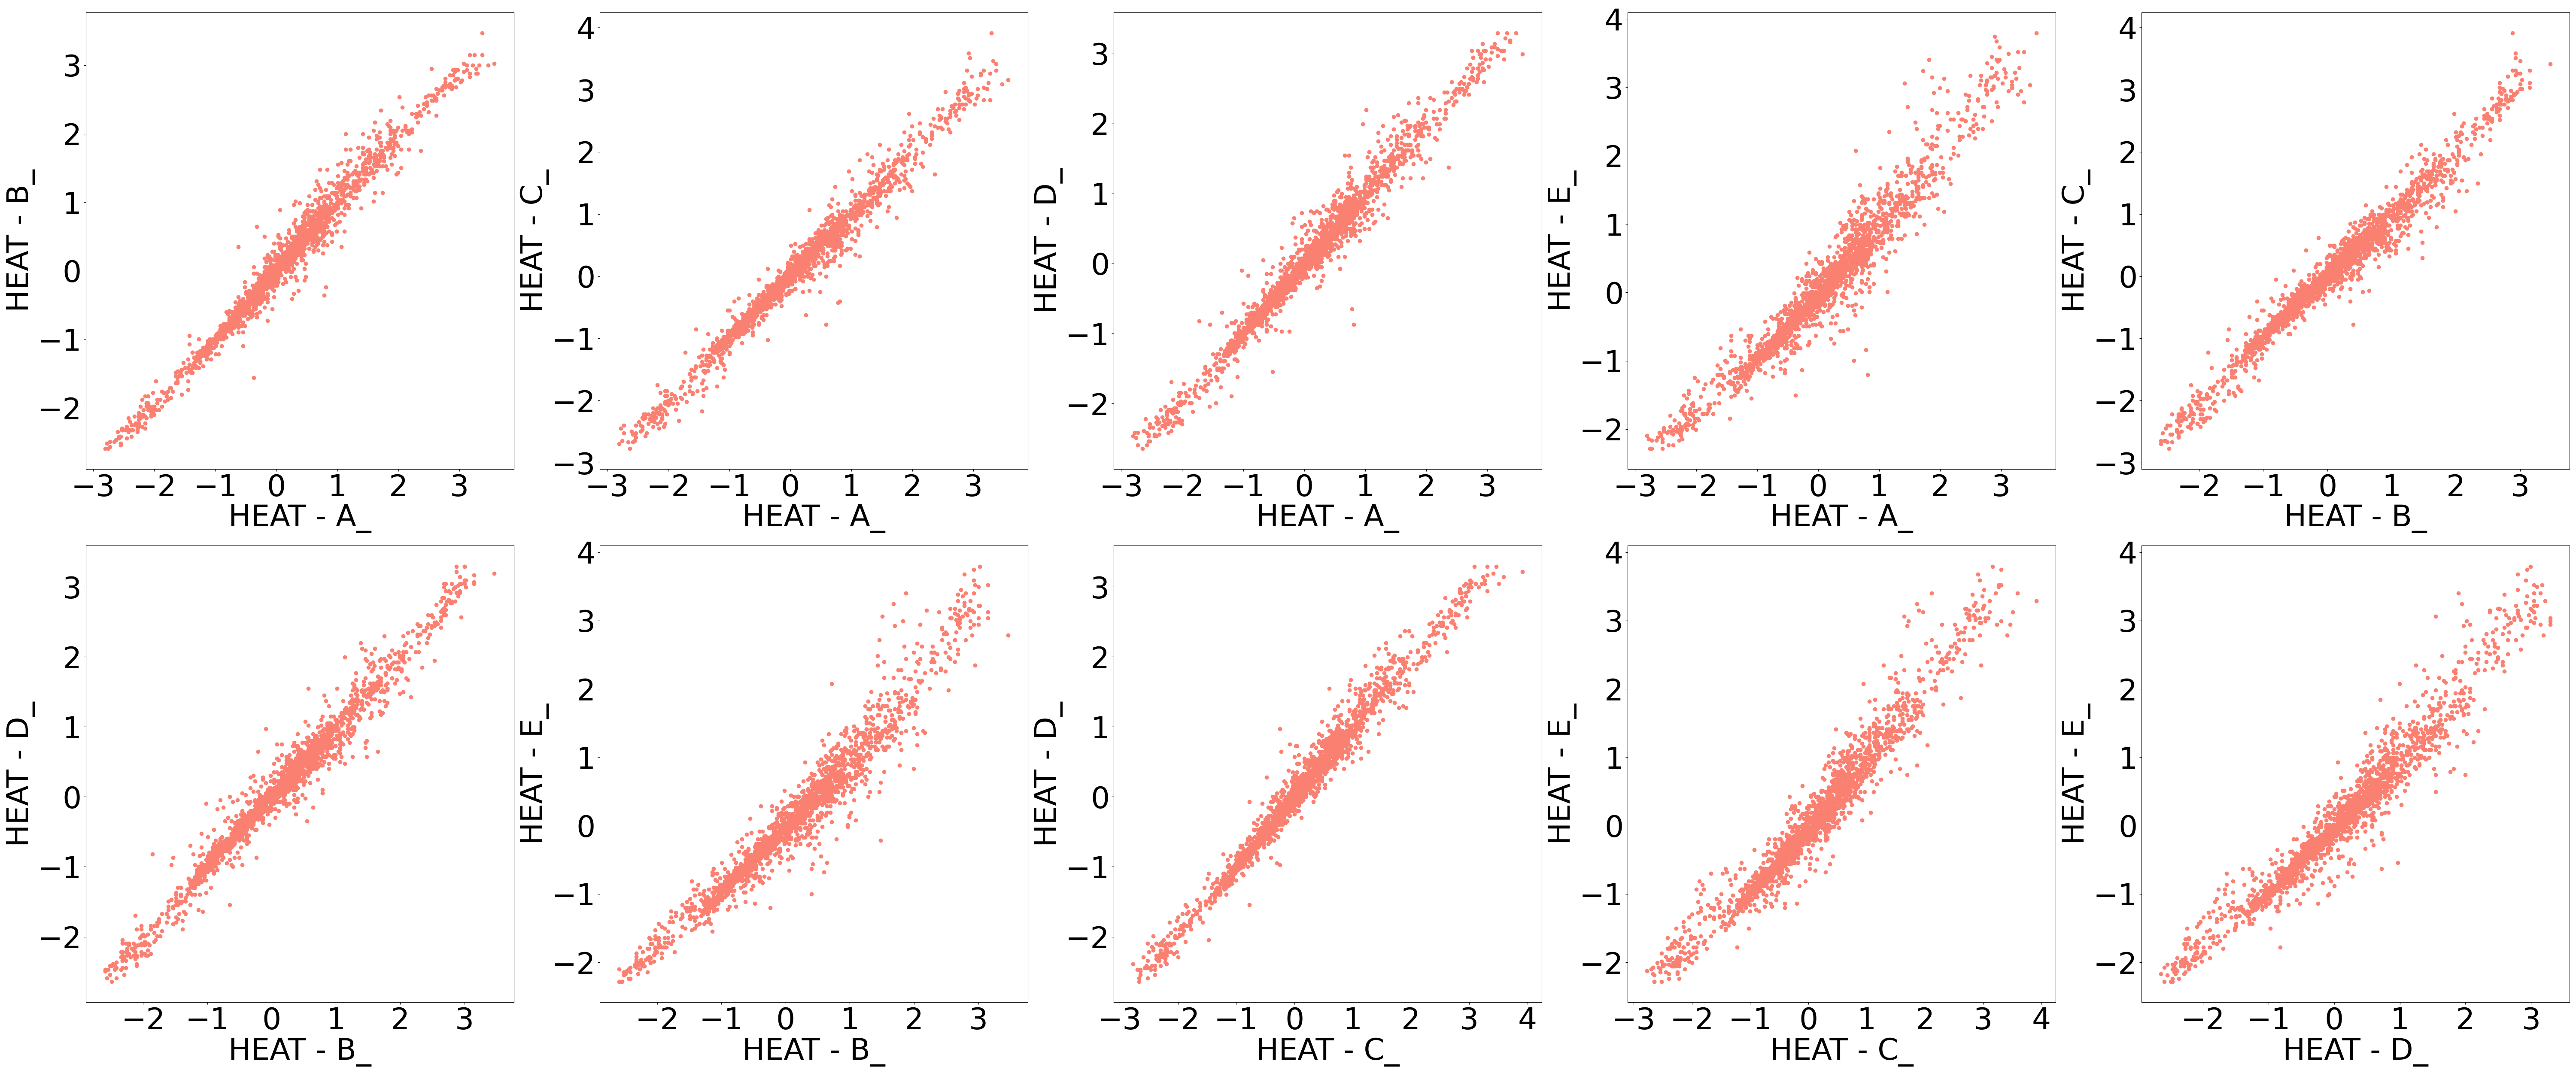
\includegraphics[width=0.9\textwidth]{images/scatter_temp.png} 
\caption{Scatter plots of Temperature values between every 2 sensors}
\end{figure}

\begin{figure}[htbp]
\centering
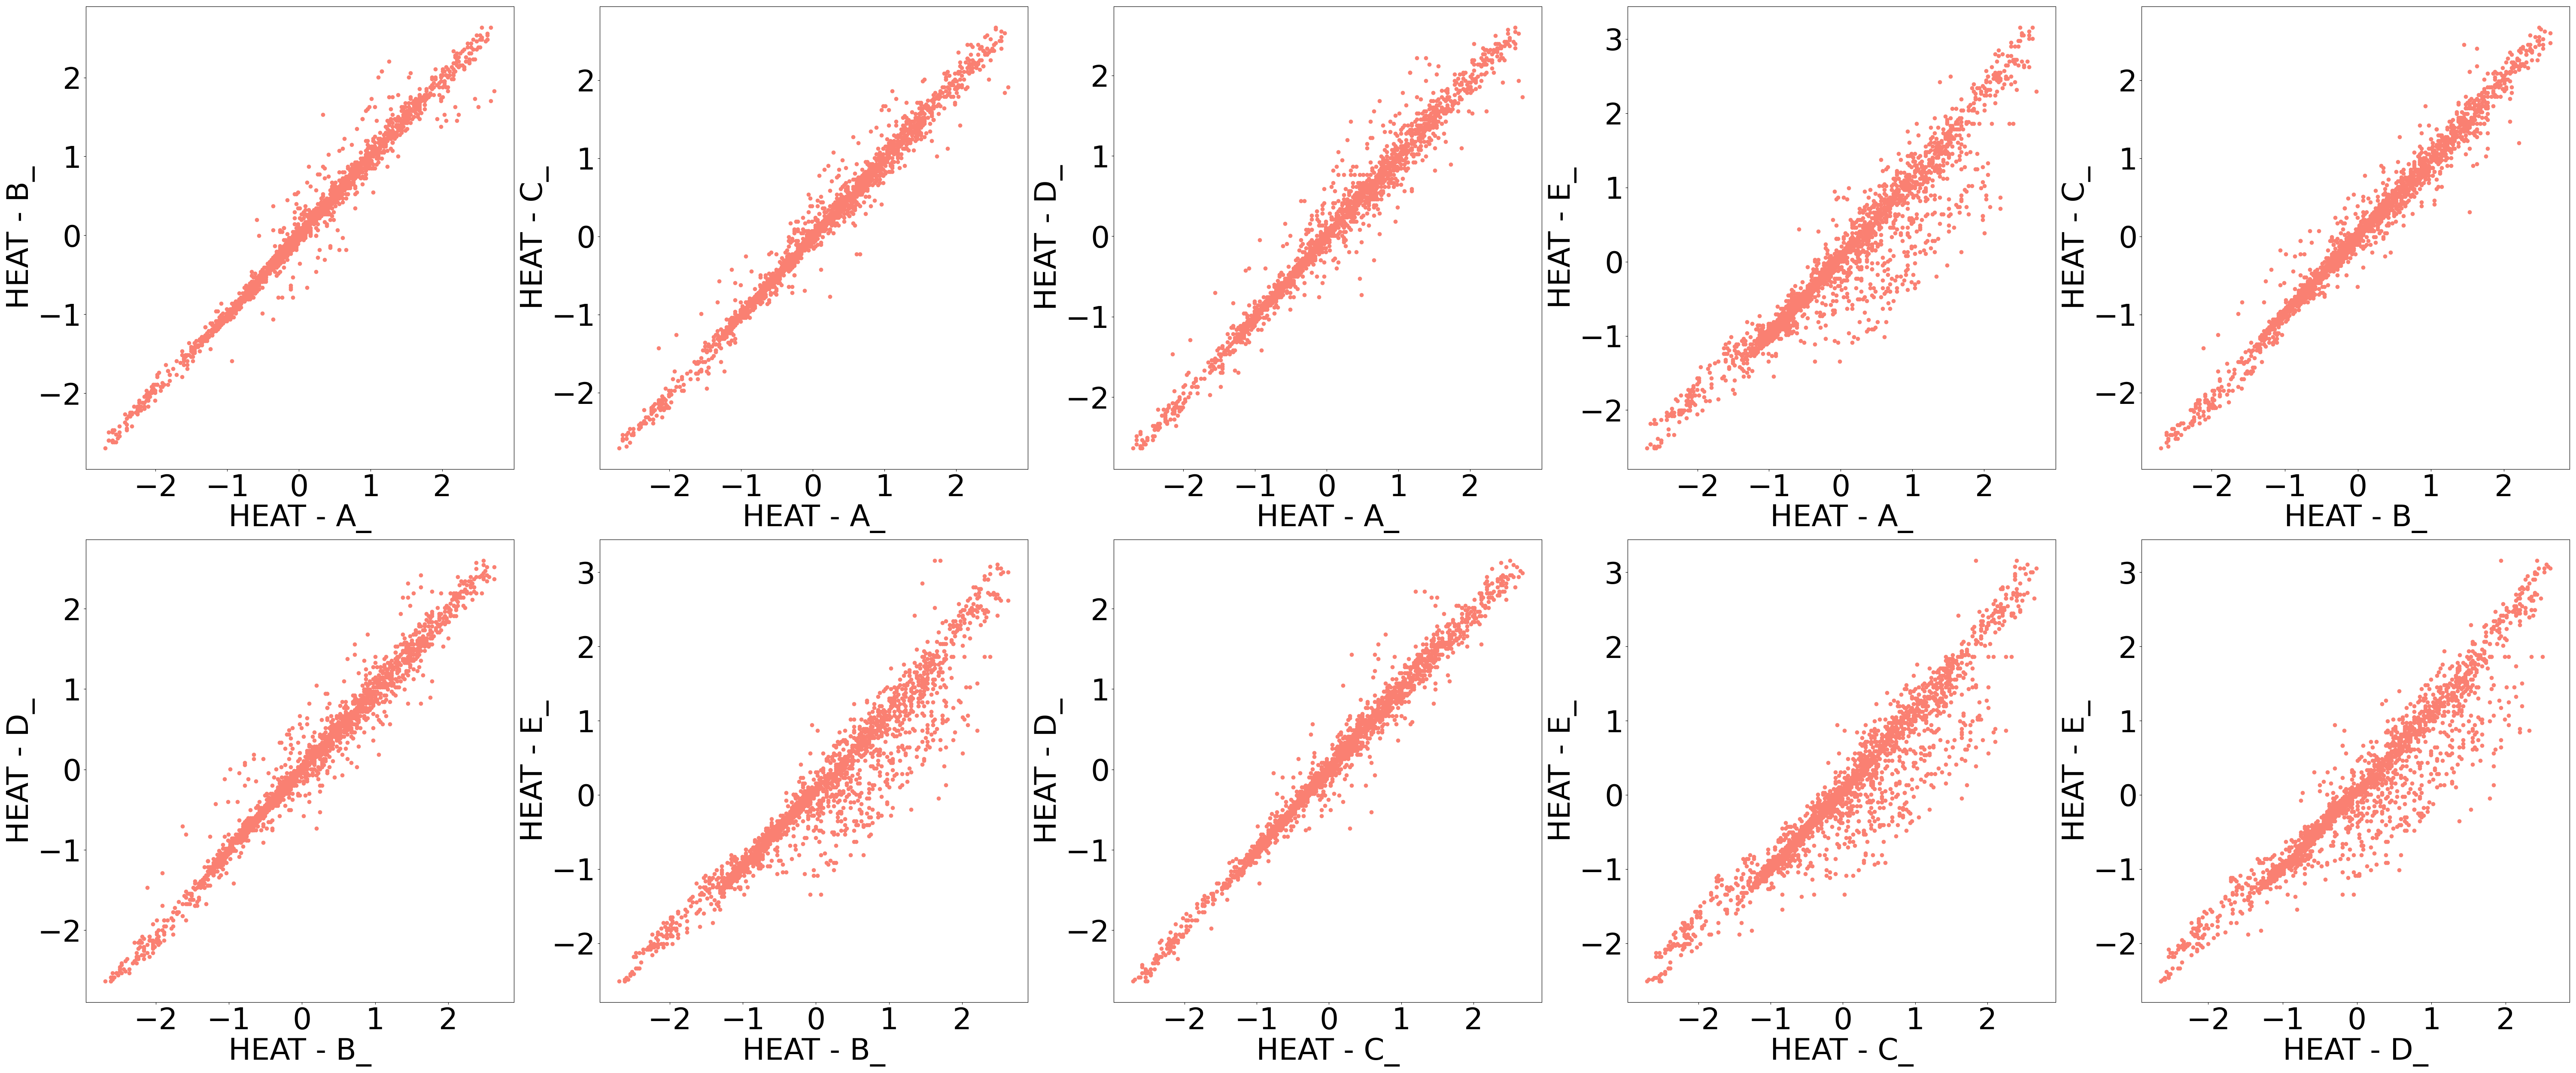
\includegraphics[width=0.9\textwidth]{images/scatter_WBGT.png} 
\caption{Scatter plots of Wet Bulb Globe Temperature (WBGT) values between every 2 sensors}
\end{figure}

\begin{figure}[htbp]
\centering
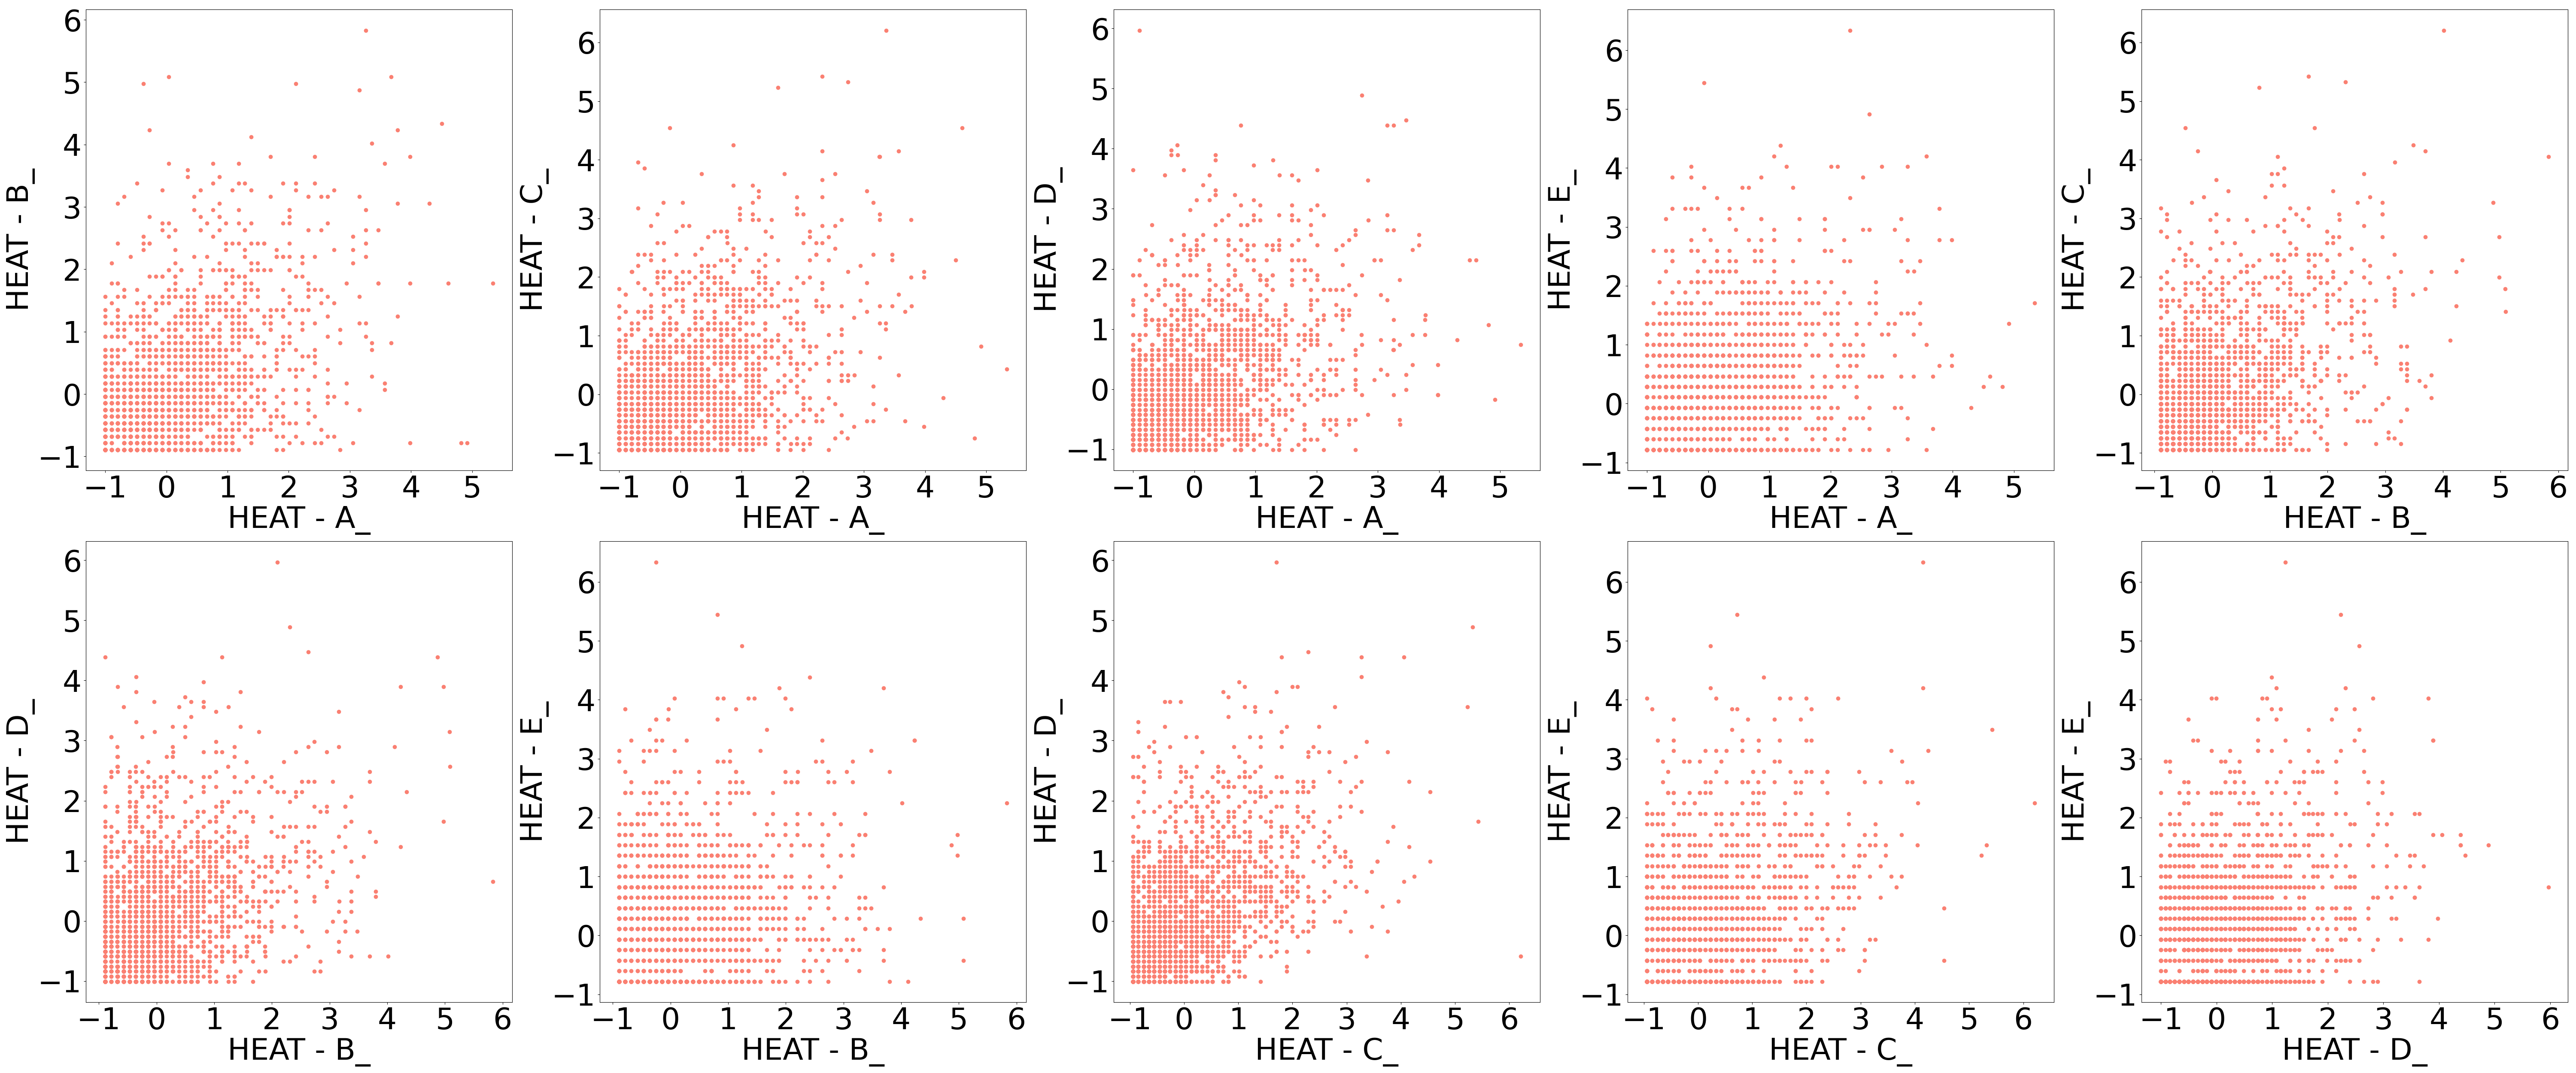
\includegraphics[width=0.9\textwidth]{images/scatter_CS.png} 
\caption{Scatter plots of Crosswind Speed values between every 2 sensors}
\end{figure}

\subsection{Question A3.2}
\noindent From \textbf{Figure 7},  \textbf{Figure 8}, \textbf{Table 4} and  \textbf{Table 5}, both the correlation coefficients and scatter plots show that 5 sensors are clearly linearly dependent in \textbf{Temperature} and \textbf{Wet Bulb Globe Temperature (WBGT)}.  

\noindent However, \textbf{Table 6} and  \textbf{Figure 9} show no obvious correlation between 5 sensors in \textbf{Crosswind Speed}.

\subsection{Question A3.3}
\noindent Calculating the mean Spearmann correlation coefficients (Pearson correlation coefficients only show the linear relation) of \textbf{Temperature} and \textbf{Wet Bulb Globe Temperature (WBGT)} of each 2 sensors. Then the following table and scatter plot can be obtained:

\begin{table}[htbp]
  \centering
  \caption{Mean values of Spearmann correlation coefficients of Temperature and Wet Bulb Globe Temperature (WBGT) of each 2 sensors}
    \begin{tabular}{c|ccccc}
          & A     & B     & C     & D     & E \\
    \midrule
    A     & 1     & 0.989756 & 0.990382 & 0.98646 & 0.960449 \\
    B     & 0.989756 & 1     & 0.987652 & 0.986712 & 0.96688 \\
    C     & 0.990382 & 0.987652 & 1     & 0.989804 & 0.963344 \\
    D     & 0.98646 & 0.986712 & 0.989804 & 1     & 0.962275 \\
    E     & 0.960449 & 0.96688 & 0.963344 & 0.962275 & 1 \\
    \end{tabular}%
\end{table}%

\begin{figure}[htbp]
\centering
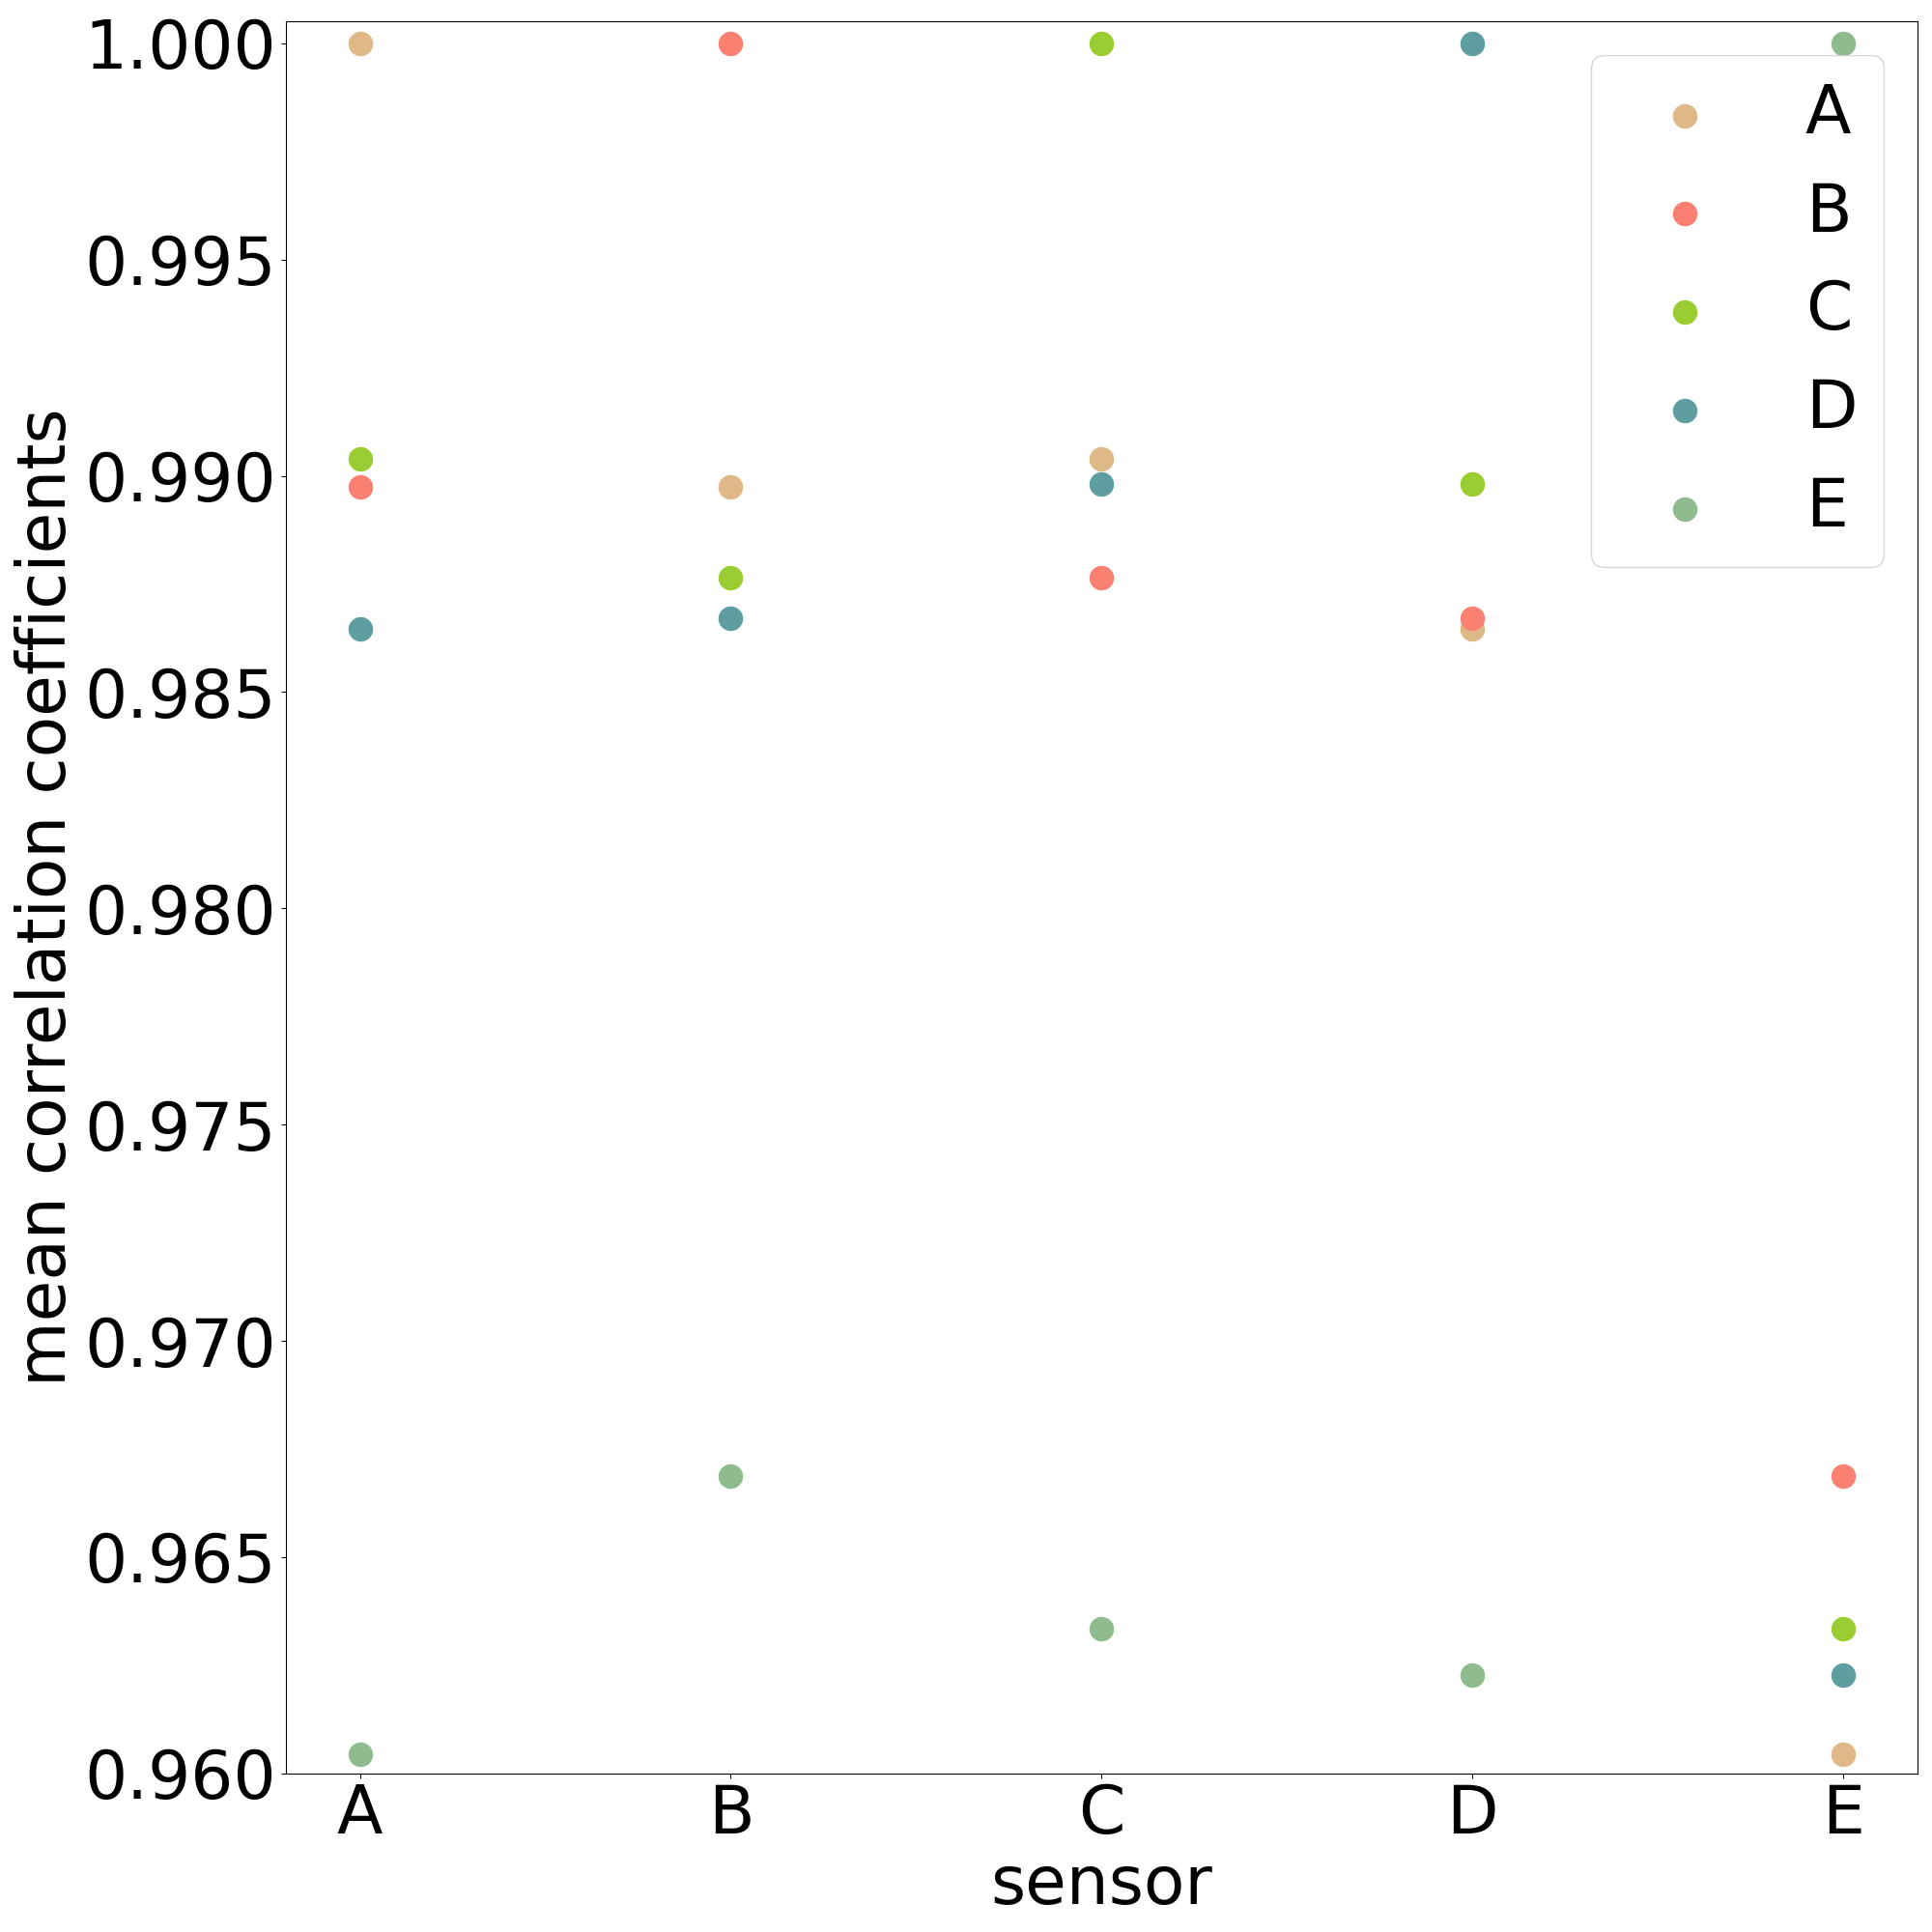
\includegraphics[width=0.5\textwidth]{images/sensors_location.png} 
\caption{Scatter plots of Mean values of Spearmann correlation coefficients of Temperature and Wet Bulb Globe Temperature (WBGT) of each 2 sensors}
\end{figure}

\begin{figure}[htbp]
\centering
\includegraphics[width=0.6\textwidth]{images/a3_3.png} 
\caption{Hypothesis conclusion}
\end{figure}

\noindent \textbf{Figure 11} show that the underlying surface may be an important factor affecting the temperature differences at several locations in the figure. Therefore, the hypothesis is mainly based on the underlying surface conditions at 5 locations and the mean Spearmann correlation coefficient of \textbf{Temperature} and \textbf{Wet Bulb Globe Temperature (WBGT)} between the five sensors. The specific hypothetical process is as follows:
\begin{enumerate}
\item Only area (4) is located on the artificial surface (with regular texture), the rest of the areas are on the natural surface. The correlations between the \textbf{sensors E} and the other sensors all are extremely low. This numerical difference may be due to the fact that the underlying surface of \textbf{sensor E} is different from other sensors. So \textbf{sensor E} should be located at location (4).
\item The column E of \textbf{Figure 10} pointed out that \textbf{sensor E} has the greatest correlation with \textbf{sensor B}. The underlying surface of area (2) is mainly soil and is close to footpaths, which makes its temperature performance closer to the artificial surface than other areas. So \textbf{sensor B} might be located at location (2).
\item The column B of \textbf{Figure 10} pointed out that \textbf{sensor B} has the greatest correlation with \textbf{sensor A}. In remote sensing images, location (5) is the soil, which is most similar to location (3).Therefore, sensor A should be in the location (5).
\item The correlation coefficient between \textbf{sensor A} and \textbf{sensor C} is also high, but the correlation coefficient between \textbf{sensor B} and  \textbf{sensor C} is not very high. So \textbf{sensor C} is likely to be located at position (1). Although it is grassland, it is small in area and close to buildings and roads, so its temperature performance may not be different from that of soil.
\item The \textbf{Figure 10} indicates that correlation coefficient between \textbf{sensor D} and \textbf{sensor C} is the highest in column D. We can speculate about that \textbf{sensor D} is situated in location (2).
\end{enumerate}

\section{Exercises after Lecture A4}
\subsection{Question A4.1}
\begin{figure}[htbp]
\centering
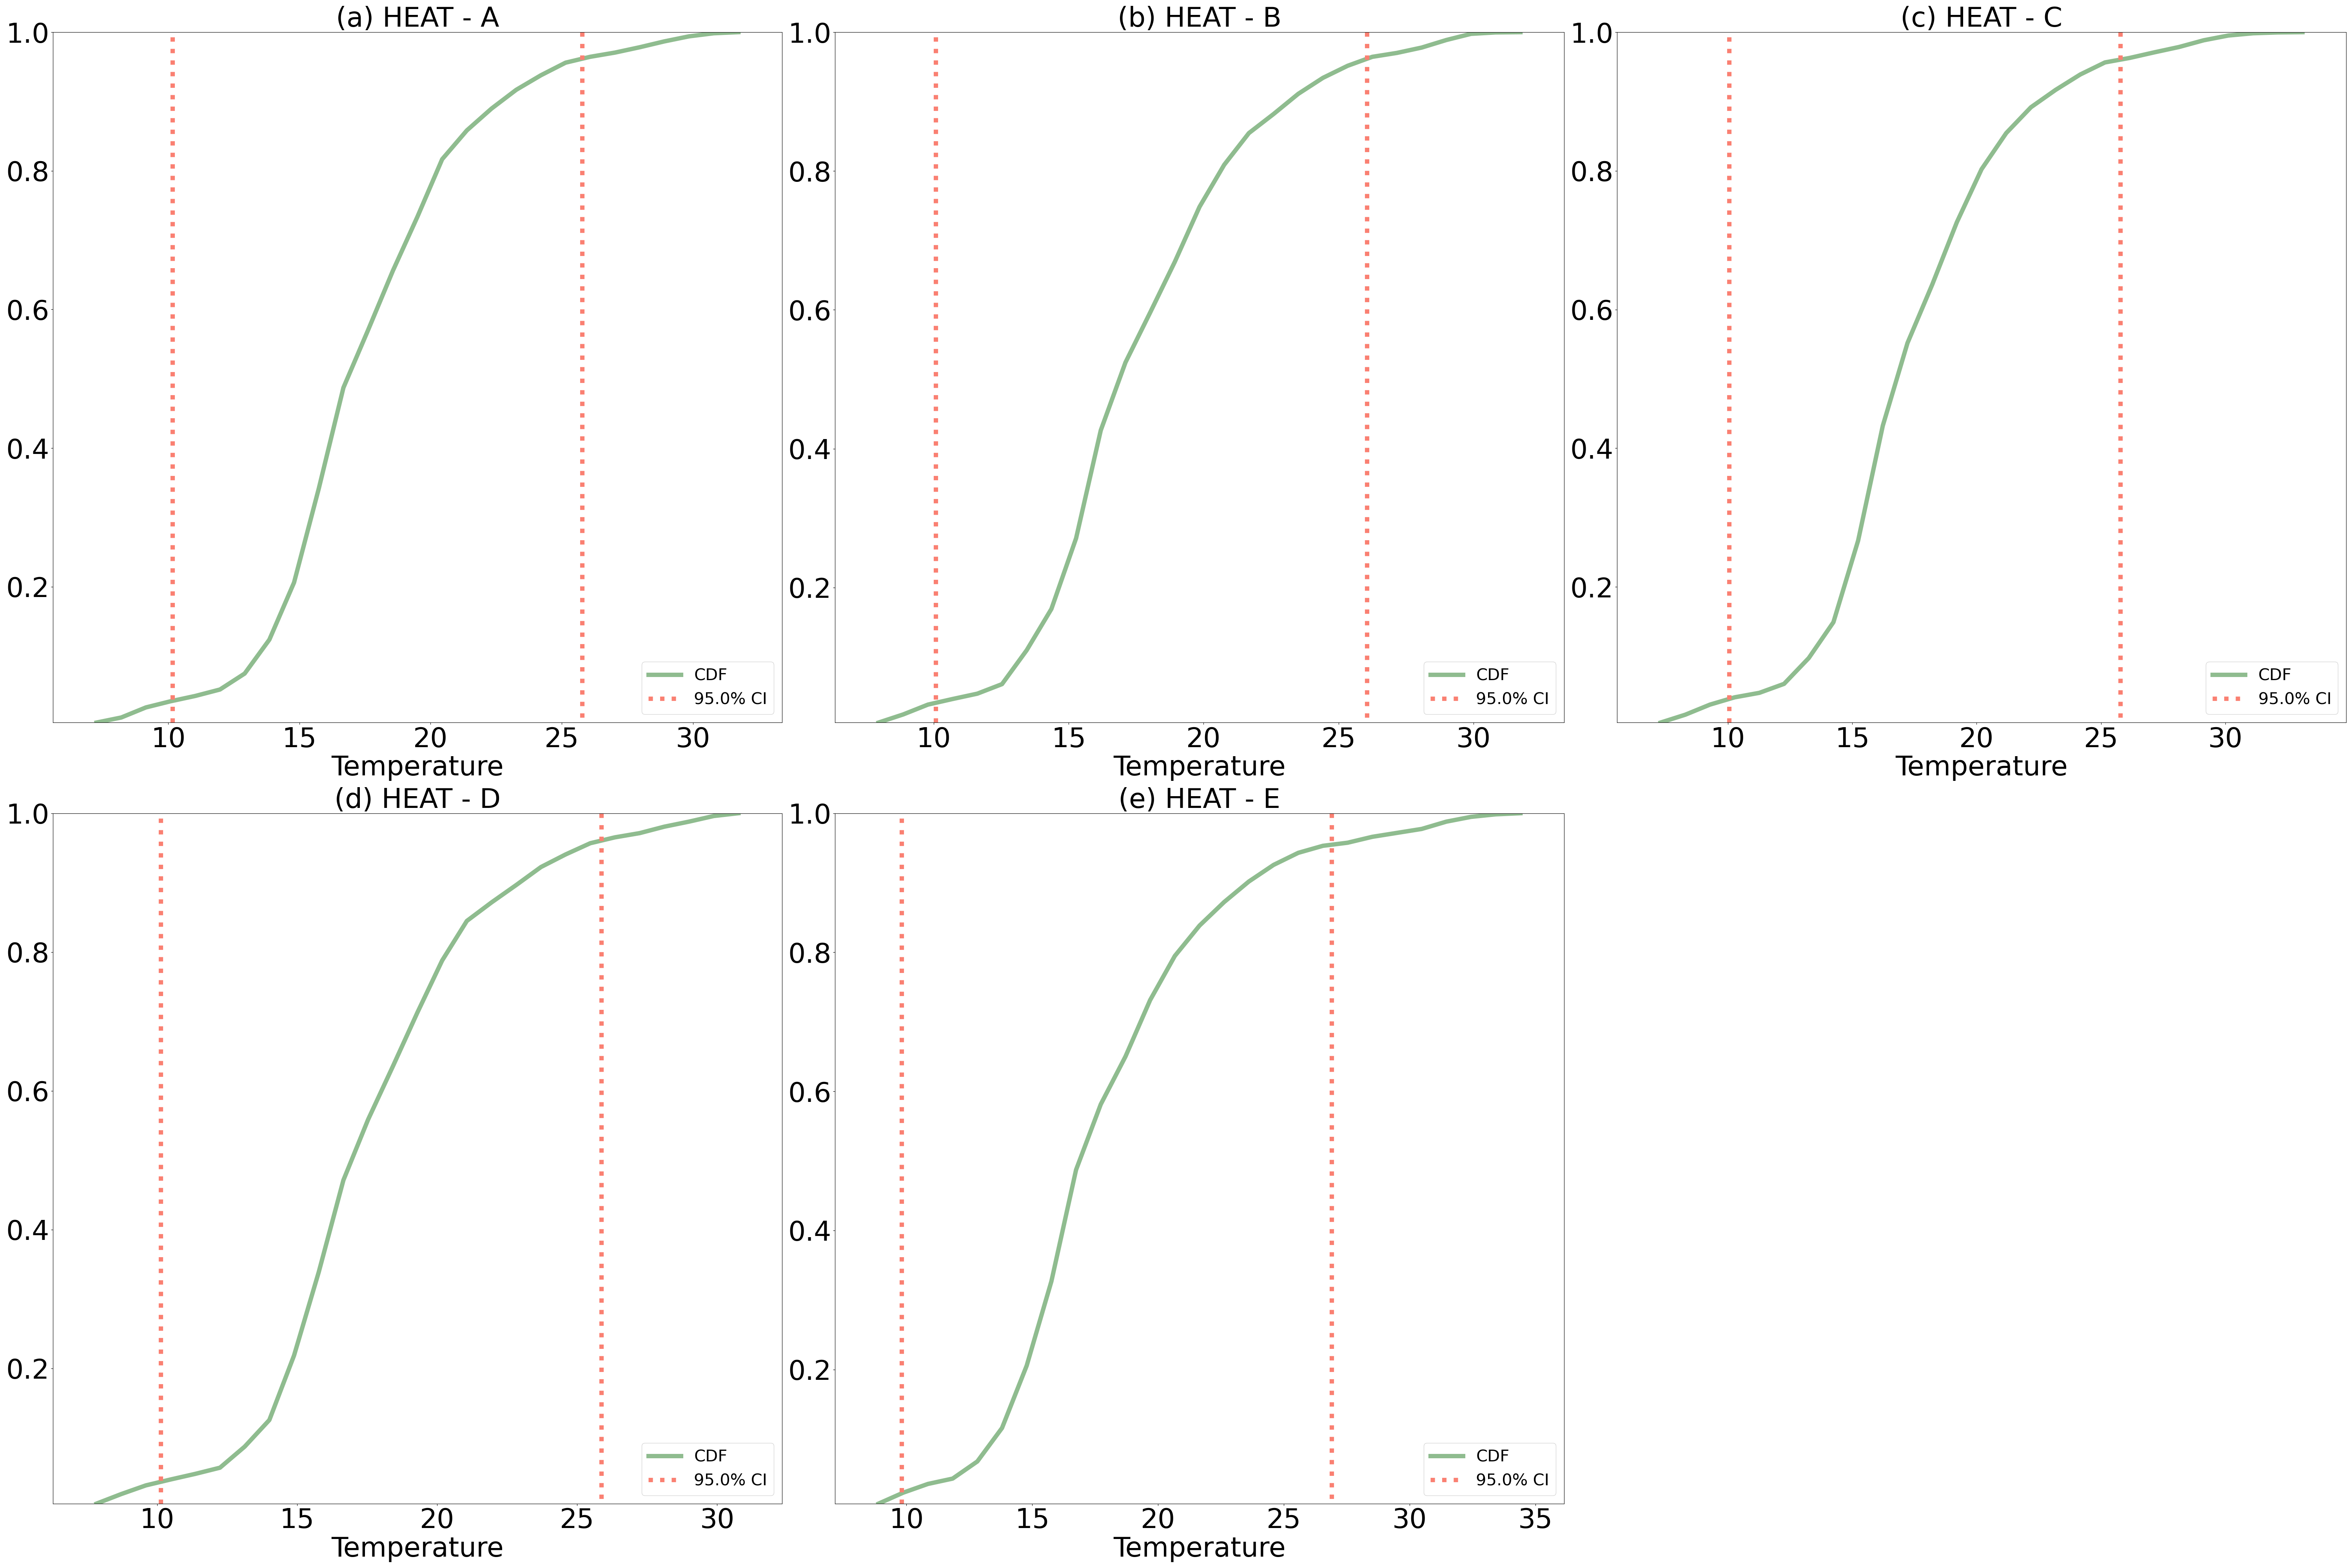
\includegraphics[width=0.7\textwidth]{images/CDF_CI_temp.png} 
\caption{CDF of Temperature values of 5 sensors with 95\% confidence intervals}
\end{figure}

\begin{figure}[H]
\centering
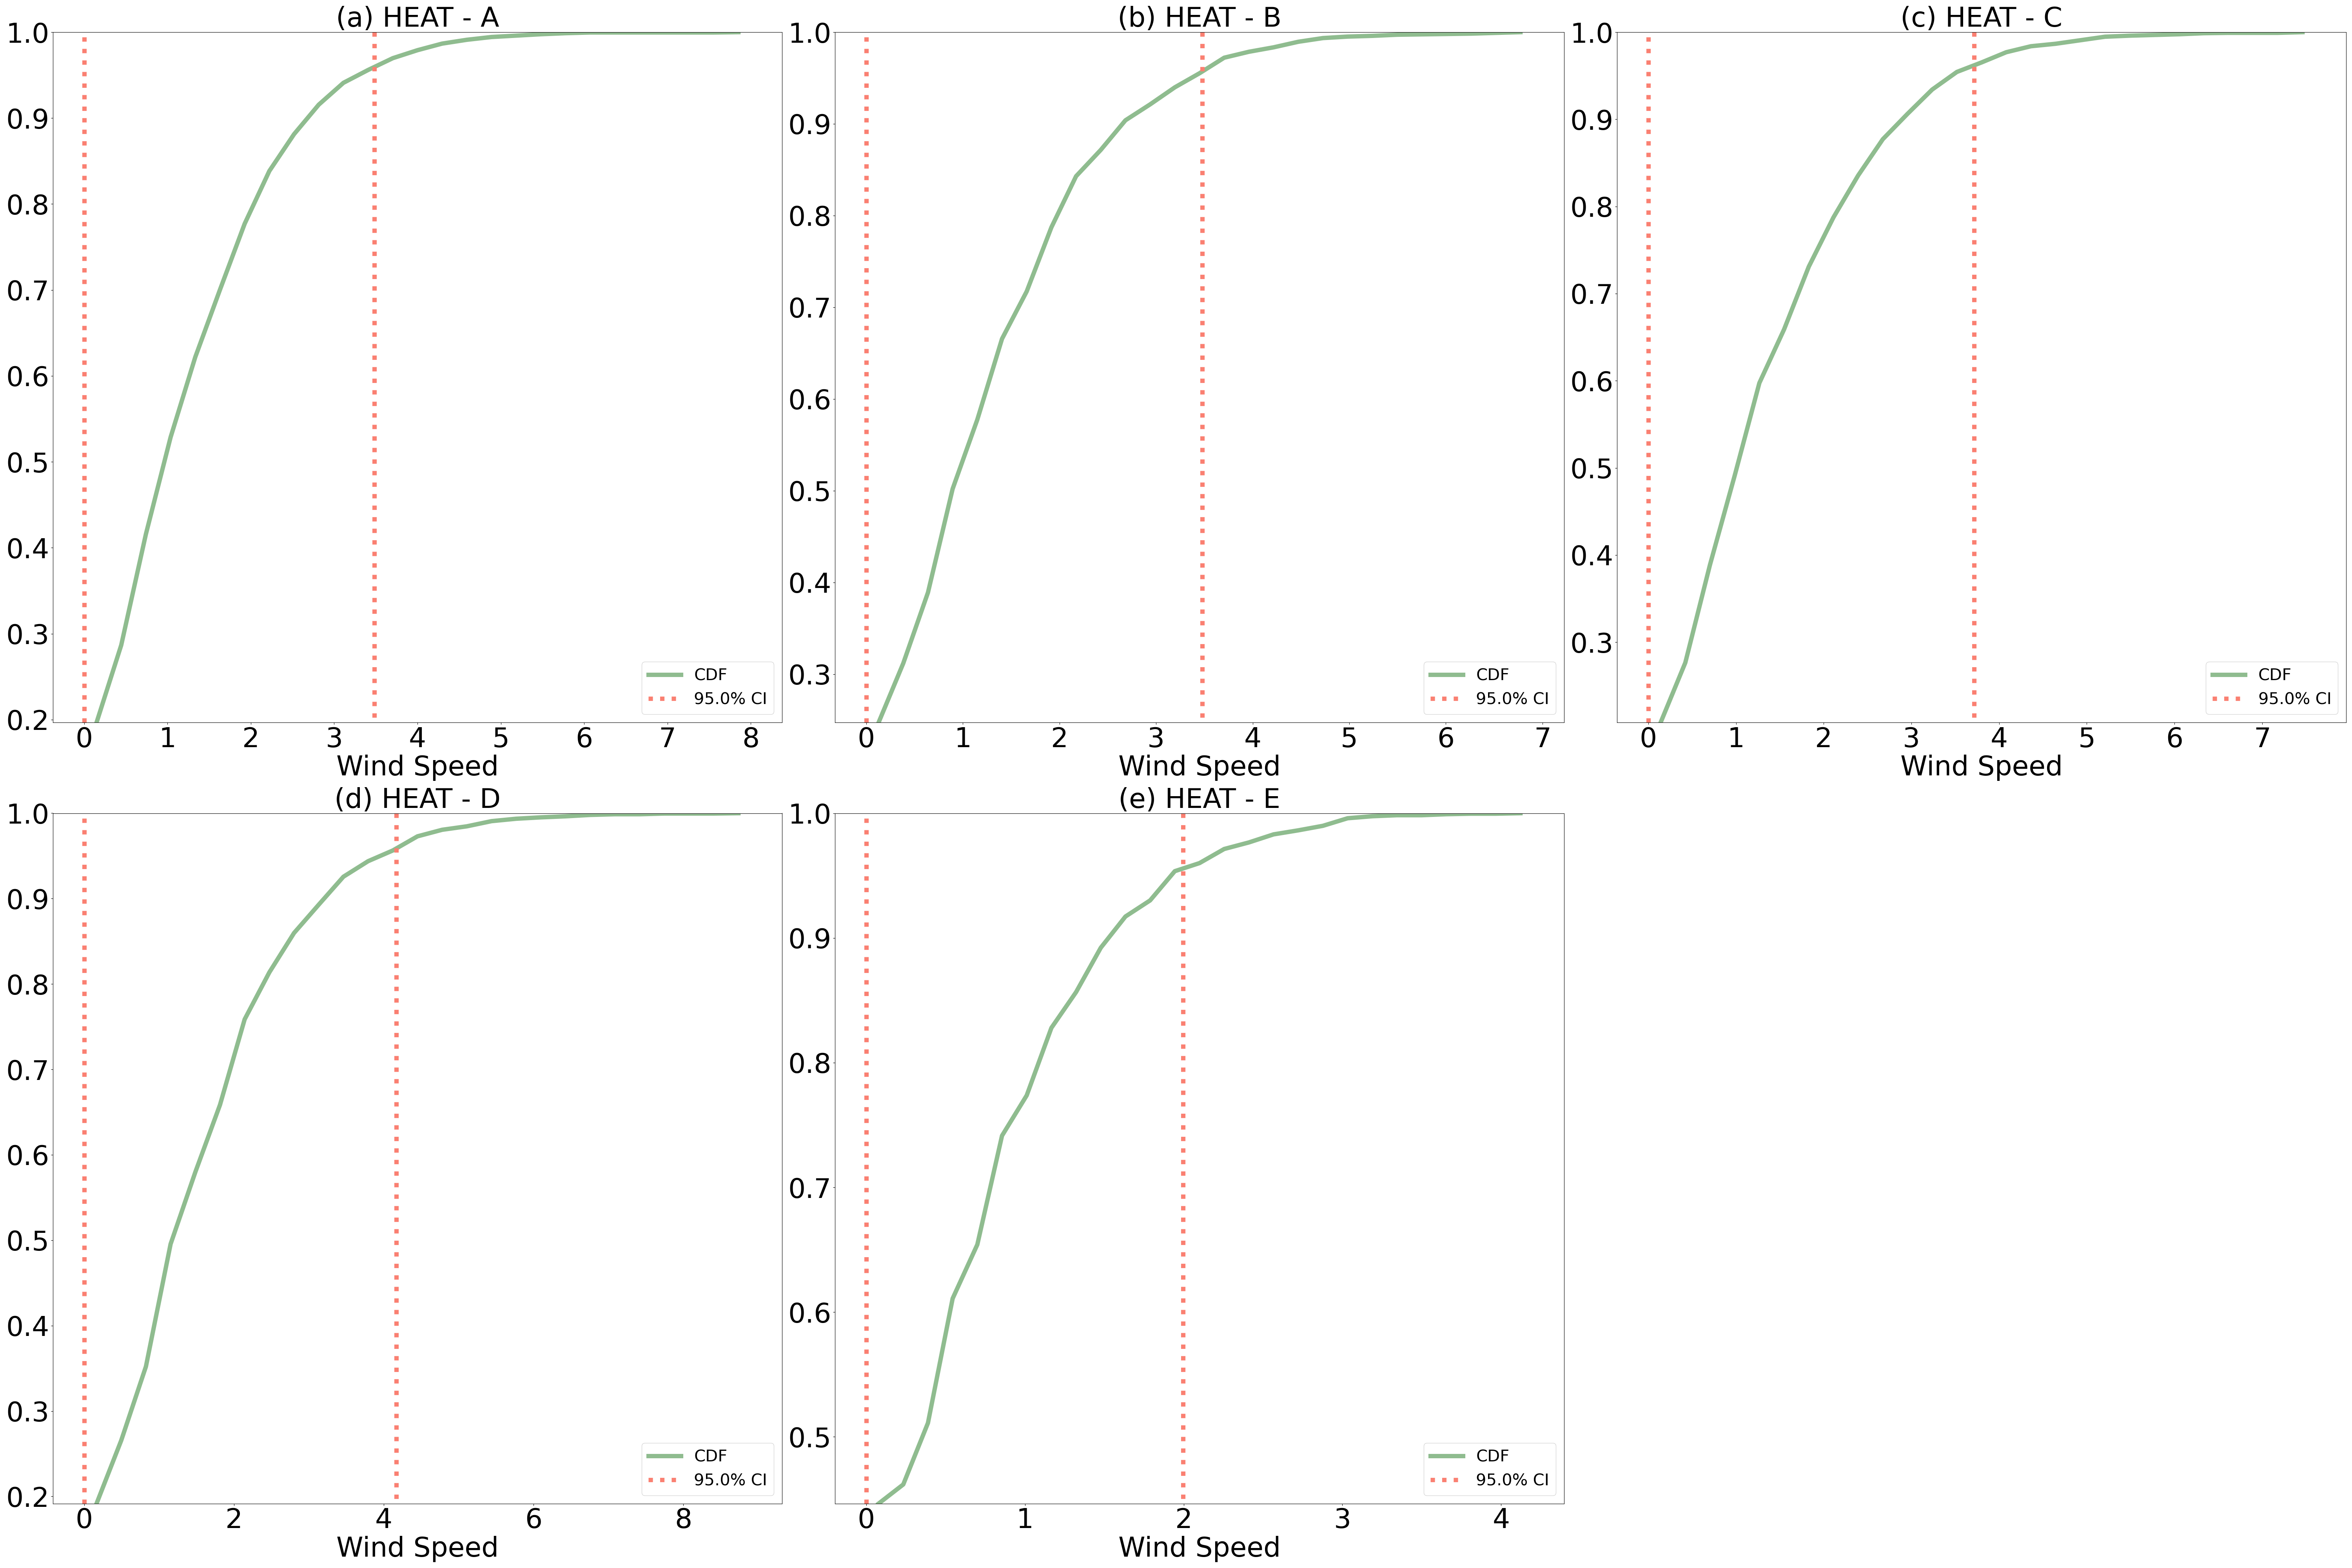
\includegraphics[width=0.7\textwidth]{images/CDF_CI_WS.png} 
\caption{CDF of Wind Speed values of 5 sensors with 95\% confidence intervals}
\end{figure}

\subsection{Question A4.2}
% Table generated by Excel2LaTeX from sheet 'A4.2'
\begin{table}[H]
  \centering
  \caption{T-Test of Temperature and Wind Speed between 2 sensors ($\alpha$=0.05)}
    \begin{tabular}{cccccc}
    \toprule
          & first sensor & second sensor & variable & t-value & p-value \\
    \midrule
    (1)   & HEAT - E & HEAT - D & Wind Speed & -32.6732 & 0 \\
    (2)   & HEAT - D & HEAT - C & Wind Speed & 5.871153 & 0 \\
    (3)   & HEAT - C & HEAT - B & Wind Speed & 3.892663 & 0.0001 \\
    (4)   & HEAT - B & HEAT - A & Wind Speed & -1.50061 & \cellcolor[rgb]{ .929,  .698,  .549}0.133519 \\
    (1)   & HEAT - E & HEAT - D & Temperature & 3.000234 & 0.002711 \\
    (2)   & HEAT - D & HEAT - C & Temperature & 0.729391 & \cellcolor[rgb]{ .929,  .698,  .549}0.465797 \\
    (3)   & HEAT - C & HEAT - B & Temperature & -1.32423 & \cellcolor[rgb]{ .929,  .698,  .549}0.185486 \\
    (4)   & HEAT - B & HEAT - A & Temperature & 0.840845 & \cellcolor[rgb]{ .929,  .698,  .549}0.400475 \\
    \bottomrule
    \end{tabular}%
  \label{tab:addlabel}%
\end{table}%


\subsection{Question A4.3}
\begin{itemize}
    \item For p-values of \textbf{Wind Speed} between \textbf{sensor E} and \textbf{D}, \textbf{sensor D} and \textbf{C}, \textbf{sensor C} and \text{B}, \textbf{Temperature} between \textbf{sensor E} and \textbf{D}, they are smaller than $\alpha$(0.05) and reject the null hypothesis. This point out that there are significant differences between these pairs of sensors.
    \item For \textbf{Wind Speed} between \textbf{sensor B} and \textbf{A} and \textbf{Temperature} between \textbf{sensor D} and \textbf{C}, \textbf{sensor C} and \textbf{B}, \textbf{sensor B} and \textbf{A}, their p-values are larger than $\alpha$(0.05). Null hypothesis is accepted, which means the differences between these pairs of sensors are not statistically significant. However, the data do not conclusively demonstrate that the null hypothesis is false.
\end{itemize}

\section{Bonus question}
\subsection{Solution}
\begin{figure}[H]
\centering
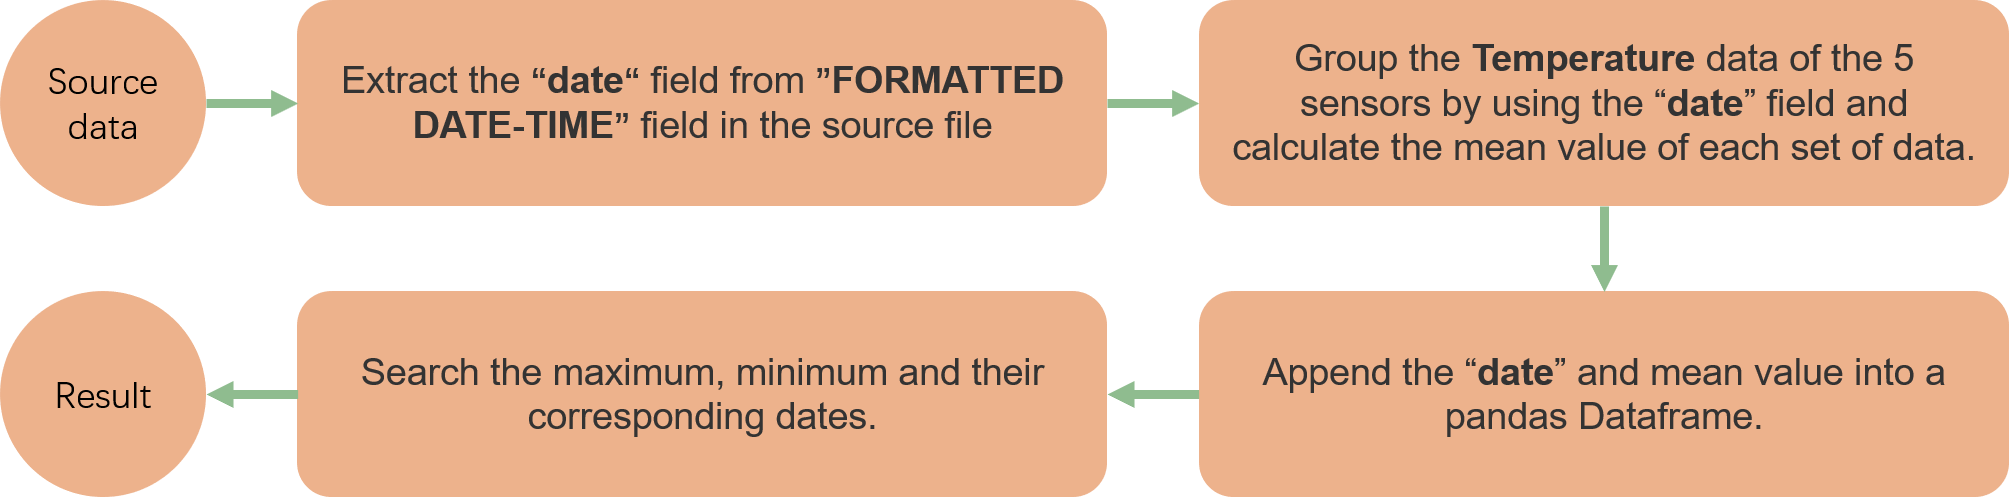
\includegraphics[width=0.8\textwidth]{images/BQ_solution.png} 
\caption{Solution of bonus question}
\end{figure}

\subsection{Conclusion}
\noindent The hottest day is \textbf{2020/6/26}, its mean temperature is \textbf{25.10361111111114°C}.  

\noindent The coldest day is \textbf{2020/6/10}, its mean temperature is \textbf{14.346944444444452°C}.

%%%%%%%% EXTRA TIPS %%%%%%%%

\bibliographystyle{plain}
\bibliography{ref}

\end{document}